\section{Exploratory Data Analysis}
Before embarking on developing statistical models and generating predictions, it
is essential to understand your data. This is typically done using conventional
numerical and graphical methods. \textcite{tukey1977exploratory} advocated the practice
of exploratory data analysis (EDA) as a critical part of the scientific process.

We present the descriptive statistics of variables in Table
\ref{tab:descriptive-statistic}

\section{Numerical Features}
\label{sec:numerical_features}
\subsection{Price}
The nightly advertised prices range from \$0 to \$10,000. The range is so broad
because hosts do not understand how to set Airbnb advertised prices.  Figure
~\ref{fig:price-distribution-1000} and Figure ~\ref{fig:price-distribution-200}
 show the distributions of price up to \$1,000 and \$200 respectively. While the
price's range is extensive, most of its values concentrate on the range \$10 to
\$1000.  Hence, for minimal values under \$10, we will increase them to \$10,
and values above \$1,000 will be reduced to \$1,000.
\begin{figure}[H]
    \centering
    \begin{subfigure}[b]{0.48\textwidth}
        \centering
        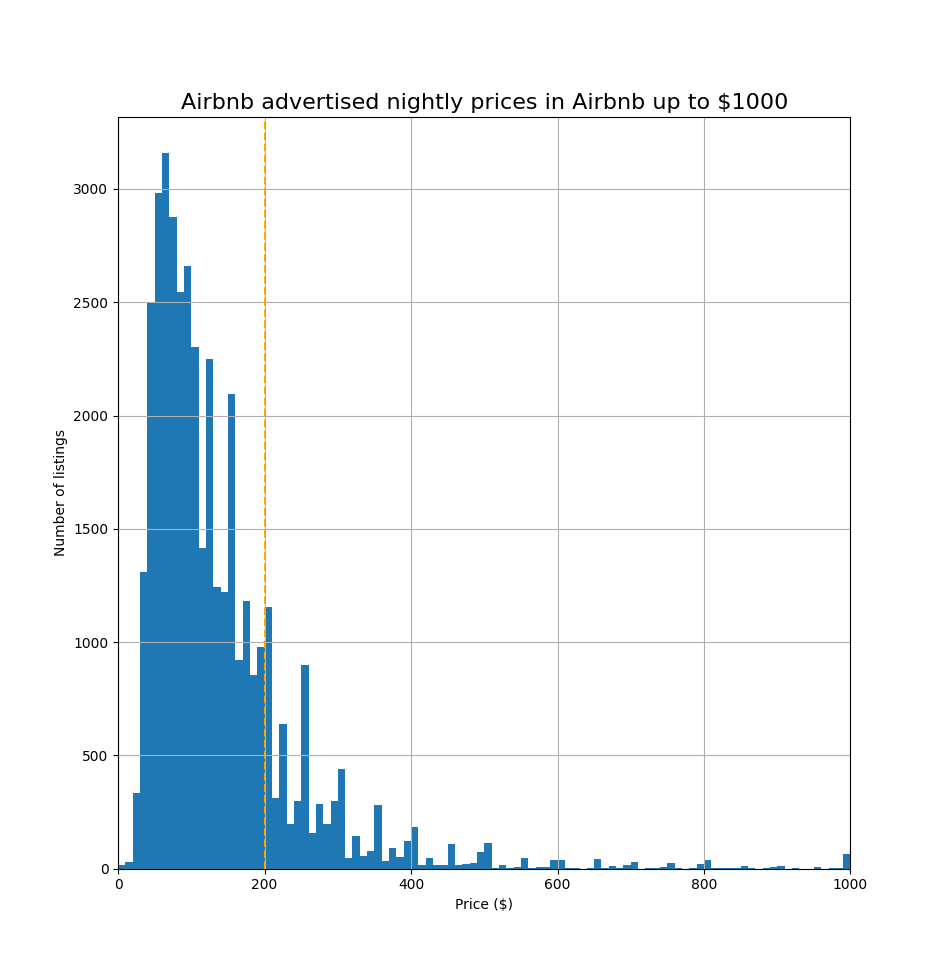
\includegraphics[width=\textwidth]{Figure_6.png}
        \caption{Airbnb advertised price up to \$1000}
        \label{fig:price-distribution-1000}
    \end{subfigure}
    \begin{subfigure}[b]{0.48\textwidth}
        \centering
        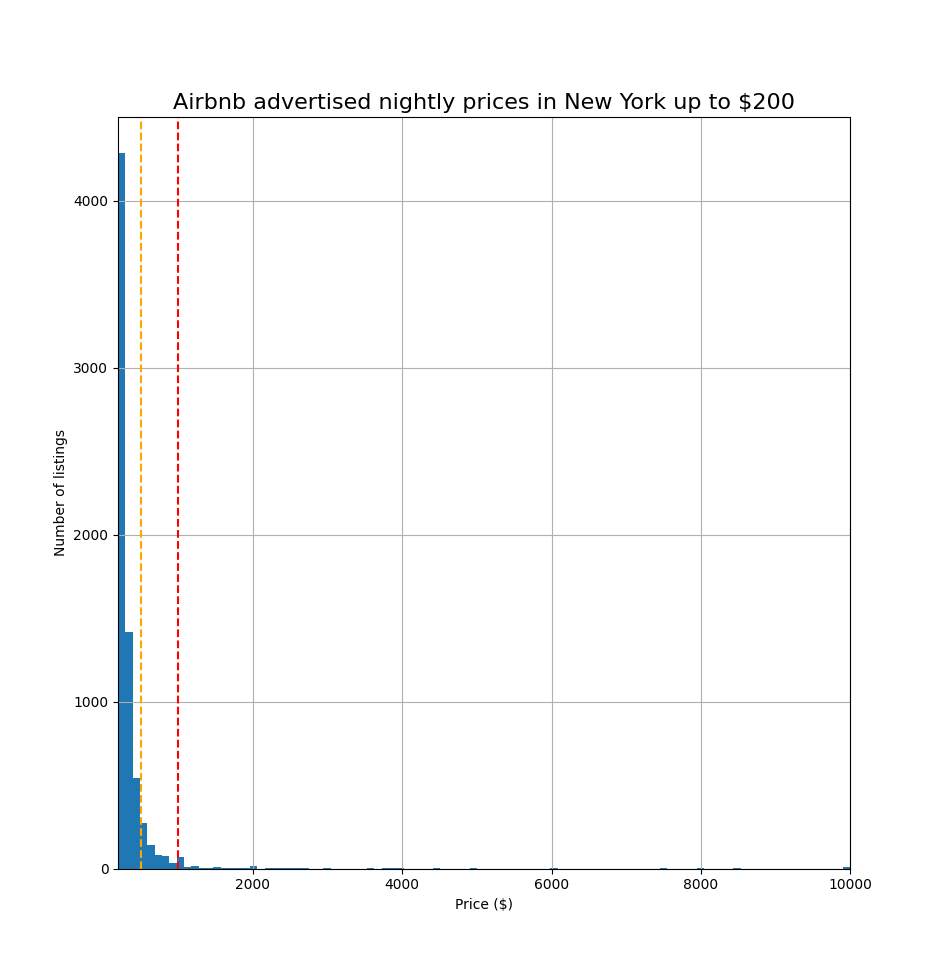
\includegraphics[width=\textwidth]{Figure_7.png}
        \caption{Airbnb advertised price up to \$200}
        \label{fig:price-distribution-200}
    \end{subfigure}
    \caption{Price Distribution}
\end{figure}

\subsection{Host Listings Count}

The median number of listings that the host of each listing has is 1. The mean
is higher (8 in total) due to some hosts running many listings. About 55\% of
listings are from hosts with one listing, and 45\% are from multi-listing hosts.
This feature has been shown to have a positive effect on the price of Airbnb
listings(\cite{chen2017consumer}, \cite{ert2016trust}, \cite{wang2017price})

\subsection{Number of people accommodated, bathrooms, bedrooms and beds}

Figure ~\ref{fig:hist-accommodates} reveals that the most common listing type accommodates two people in
one bed in one bedroom with one bathroom.

\begin{figure}[H] \centering
    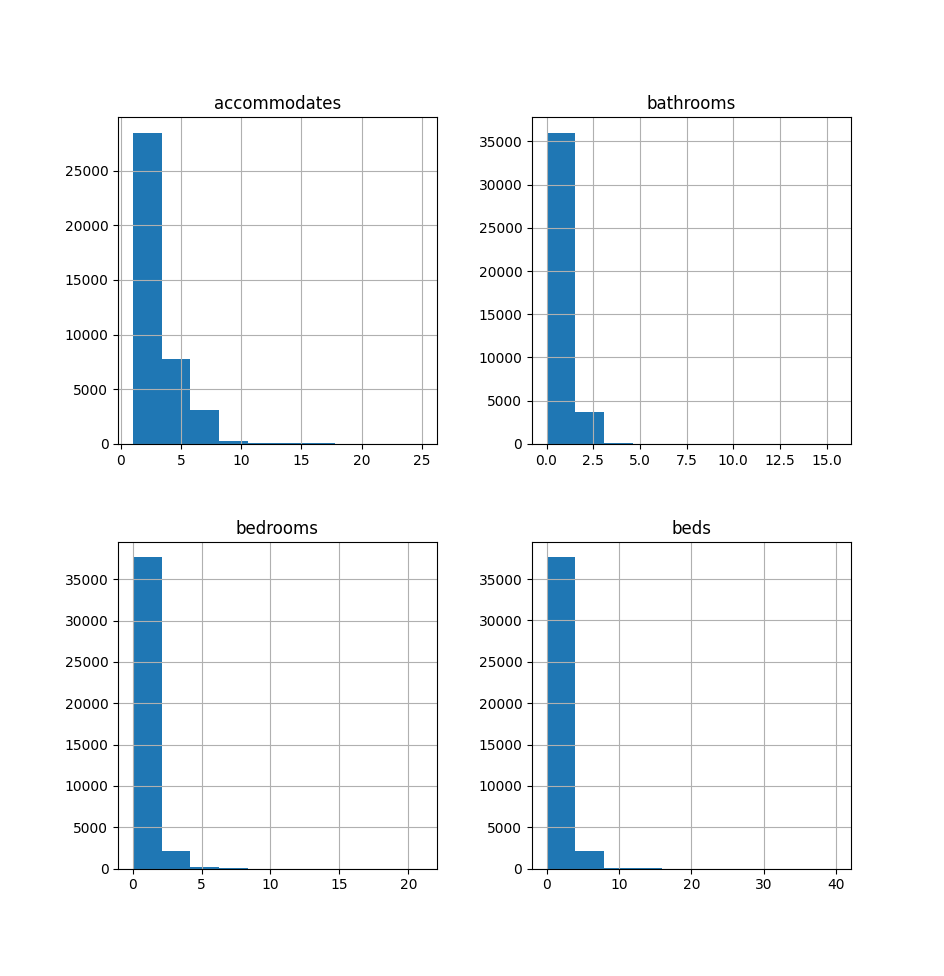
\includegraphics[width=\textwidth]{Figure_9.png}
    \caption{Histogram Plot of Accomodate, Bathrooms, Bedrooms, and Beds}
    \label{fig:hist-accommodates}
\end{figure}


The number of bedrooms, number of bathrooms, and number of accommodations appear
to have a positive impact on Airbnb rental price (\cite{ert2016trust};
\cite{chen2017consumer}; \cite{wang2017price}; \cite{gibbs2018use}). Figure
\ref{fig:accommodates-bedrooms-bathrooms} shows that the more people a listing
accommodates, the more number of bedrooms it has, the more bathrooms it has, the
higher the price they can charge their customers. However, we can see that those
figures' general trends are similar, which implies that those features may be
highly correlated.

\begin{figure}[H]
    \centering
    \begin{subfigure}[b]{0.48\textwidth}
        \centering
        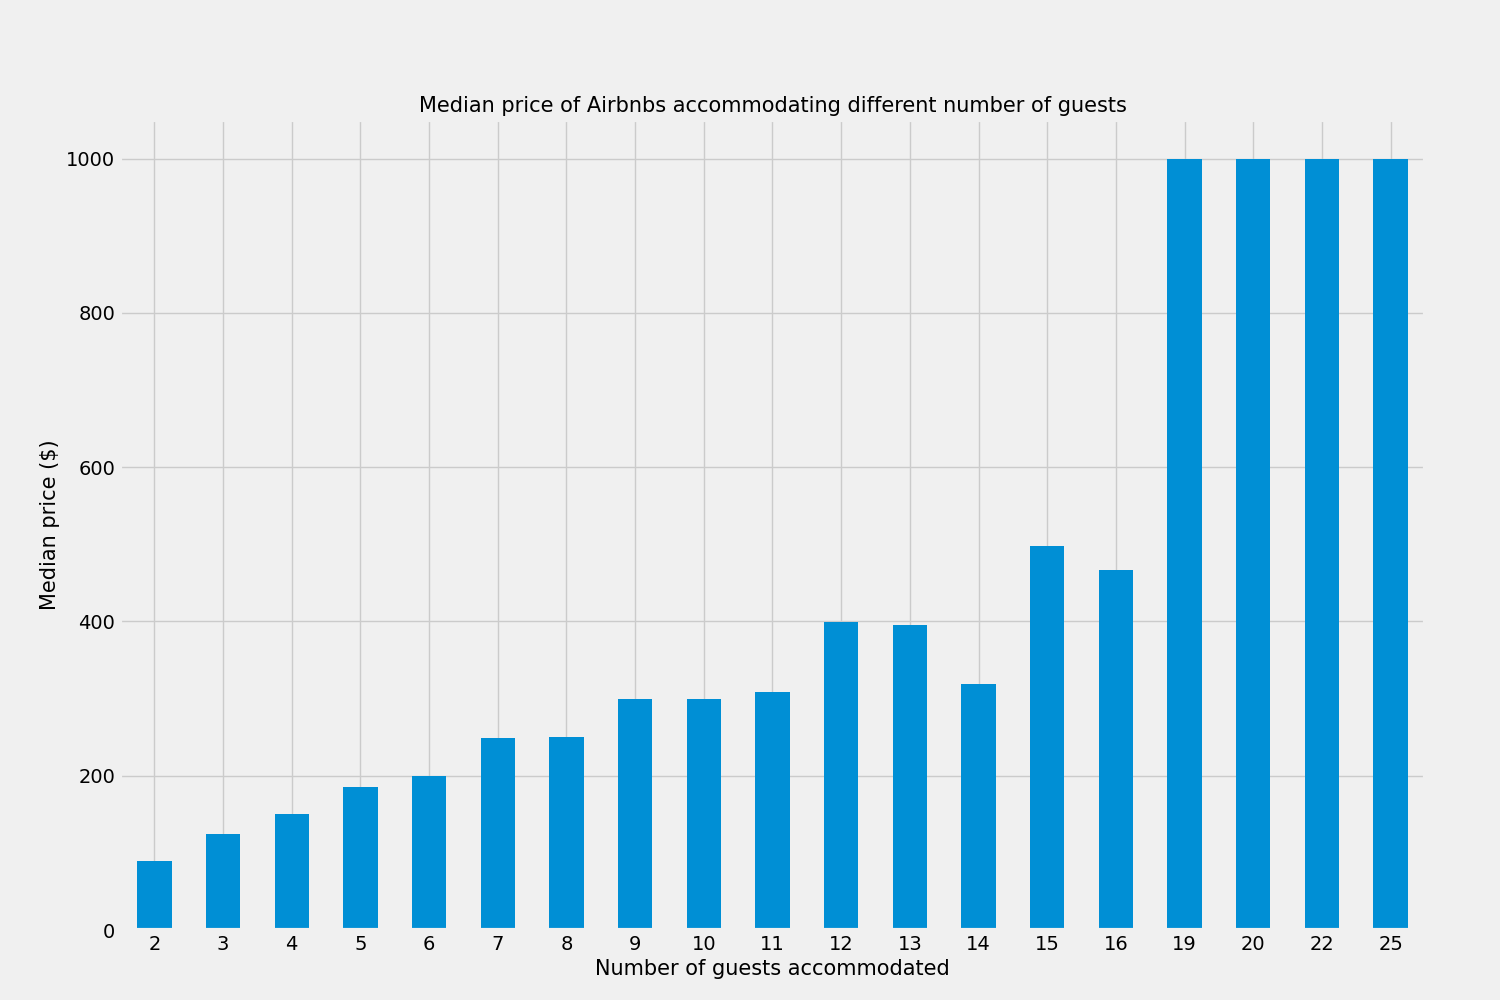
\includegraphics[width=\textwidth]{Figure_8.png}
        \caption{Accomodates}
        \label{fig:median-price-by-accommodates}
    \end{subfigure}
    \begin{subfigure}[b]{0.48\textwidth}
        \centering
        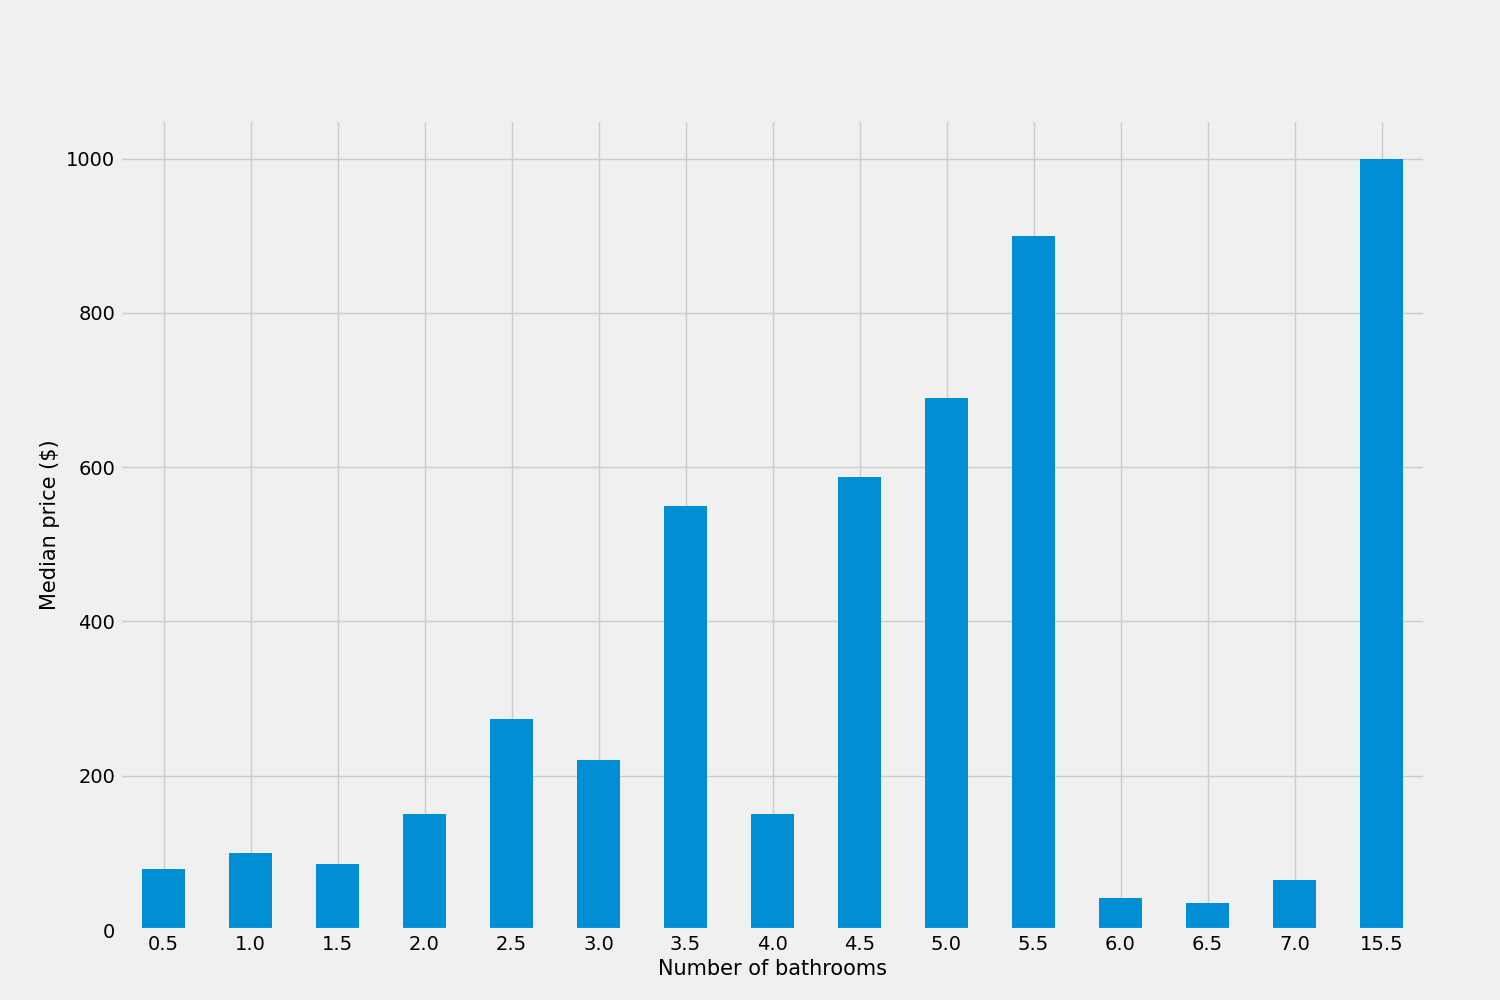
\includegraphics[width=\textwidth]{Figure_8_b.png}
        \caption{Number of Bedrooms}
        \label{fig:median-price-by-number-of-bedrooms}
    \end{subfigure}
    \begin{subfigure}[b]{0.48\textwidth}
        \centering
        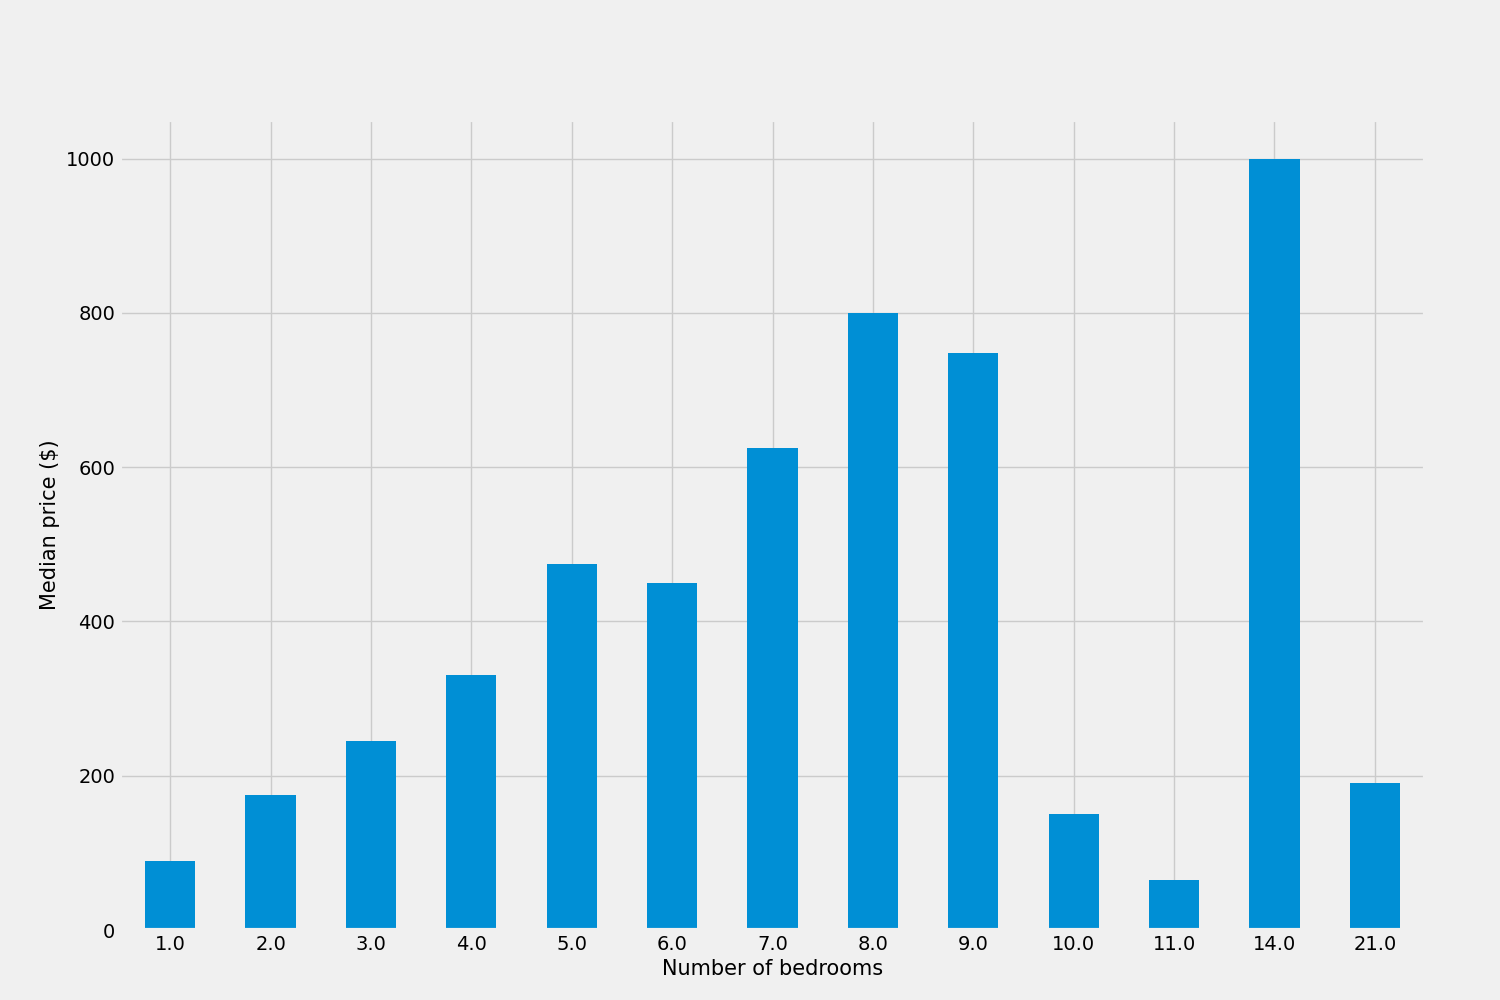
\includegraphics[width=\textwidth]{Figure_8_c.png}
        \caption{Number of Bathrooms}
        \label{fig:median-price-by-number-of-bathrooms}
    \end{subfigure}
    \caption{Median Rental Price by the Accomodates, Number of Bedrooms, and Bathrooms}
    \label{fig:accommodates-bedrooms-bathrooms}
\end{figure}

\section{Categorical features}
\label{sec:categorical_features}

Our main EDA objective for categorical data is to know the unique values and
their corresponding count.

\subsection{Neighbourhood}

Several numbers of published studies recognize the importance of locational
factors in the pricing strategy of Airbnb.  A listing close to the city center
(\cite{gibbs2018use};\cite{li2016pros}; \cite{wang2017price};
\cite{zhang2017key};\cite{gibbs2018use}) and coastline (\cite{perez2018and}) has
a higher room rate.  \cite{perez2018and} also found that a listing located
within sightseeing, eating, or shopping area gains a price premium.

As shown in Figure \ref{fig:borough-number-of-listing} and Figure
\ref{fig:borough-price-distribution}, Manhattan and Brookly have most Airbnb
properties are the most expensive boroughs, which is not surprising because they
are the famous tourist attractions.  In those two boroughs, tourists can find
neighborhoods for almost any interest. For example:

\begin{itemize}
  \item Sightseeing: Midtown is the heart of New York shopping and theater and
    home to some of its most iconic buildings.
  \item Nightlife:  More clubs are found in “Hell’s Kitchen,”
  \item Food: In Soho, tourists can experience a host of the highest-rated
    dining places.
  \item Theather: There is no more convenient home base than
    the Theater District,  located in 42nd Street to 50th Street west of Sixth
    Avenue.
  \item For families: Upper West Side is bordered with parks and playgrounds and
  boasting both a children’s museum and the famed dinosaurs at the American Museum
  of Natural. This neighborhood is also considered one of the safest areas of New
  York City
\end{itemize}


\begin{figure}[H] \centering
    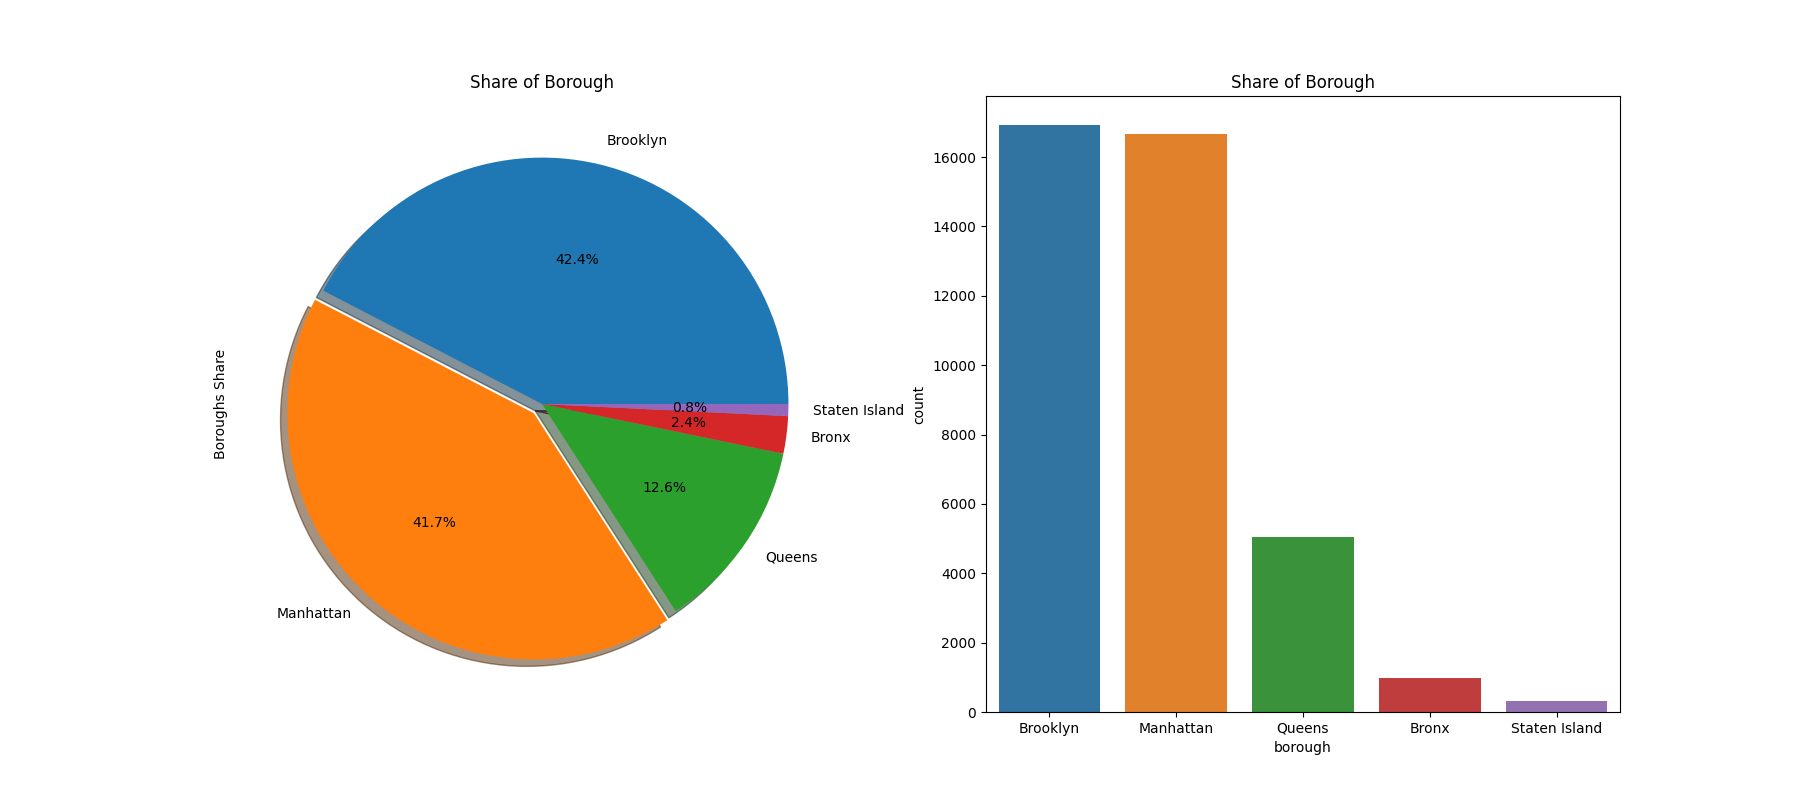
\includegraphics[width=\textwidth]{Figure_10_b.png}
    \caption{Borough Listings}
    \label{fig:borough-number-of-listing}
\end{figure}

Figure below reveal top ten neighbourhood with most listings:
\begin{figure}[H] \centering
    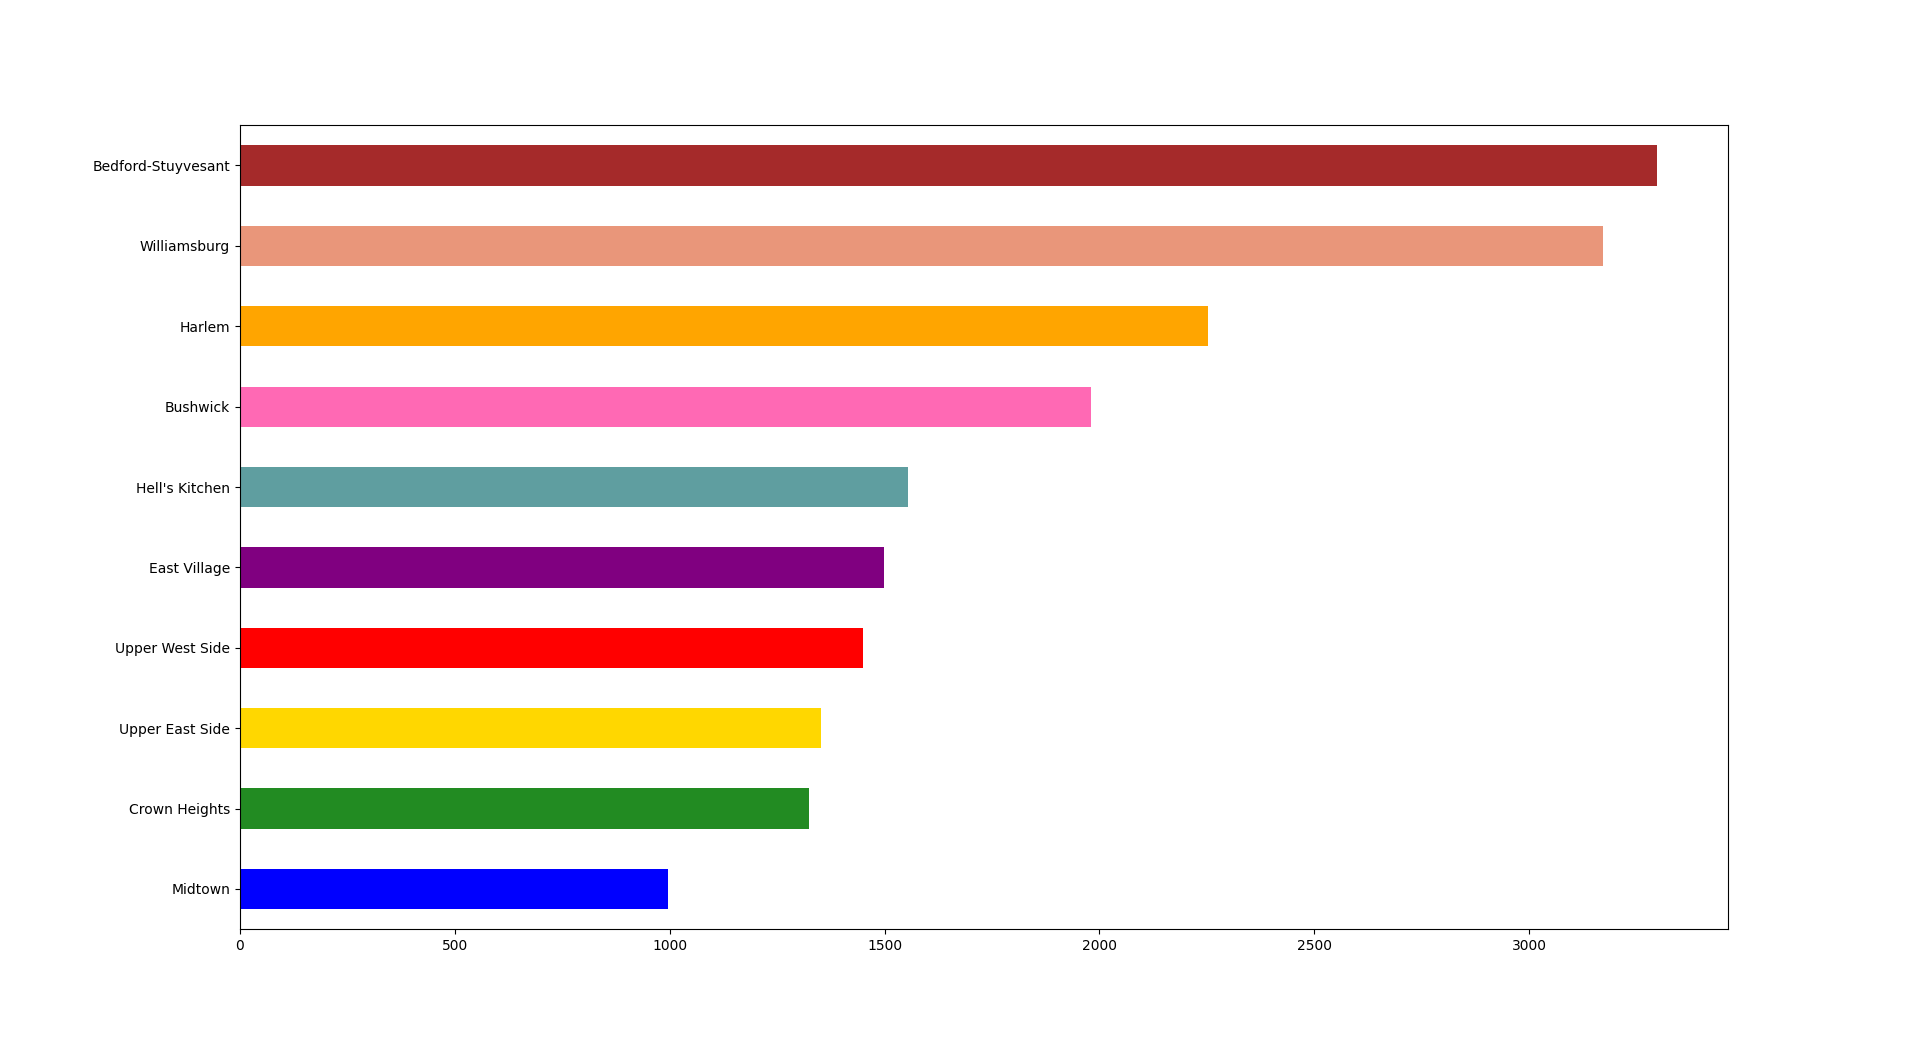
\includegraphics[width=\textwidth]{Figure_10_c.png}
    \label{fig:top-ten-most-listing-neighbourhood}
    \caption{Top 10 Neighbourhood with Most Listings}
\end{figure}



%\begin{figure}[H]\centering
    %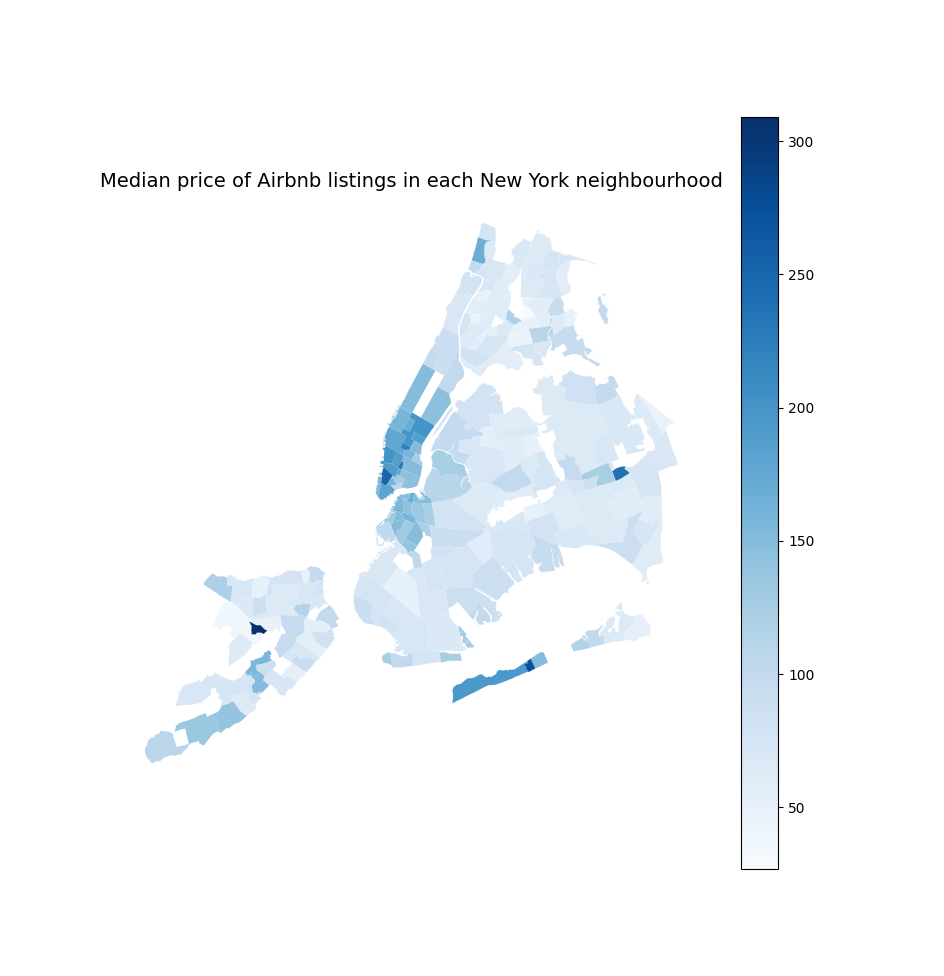
\includegraphics[width=0.75\textwidth]{Figure_11.png}
    %\caption{Median Price of Airbnb listings in each New York borough}
    %\label{fig:median-price-borough}
%\end{figure}

\begin{figure}[H]\centering
    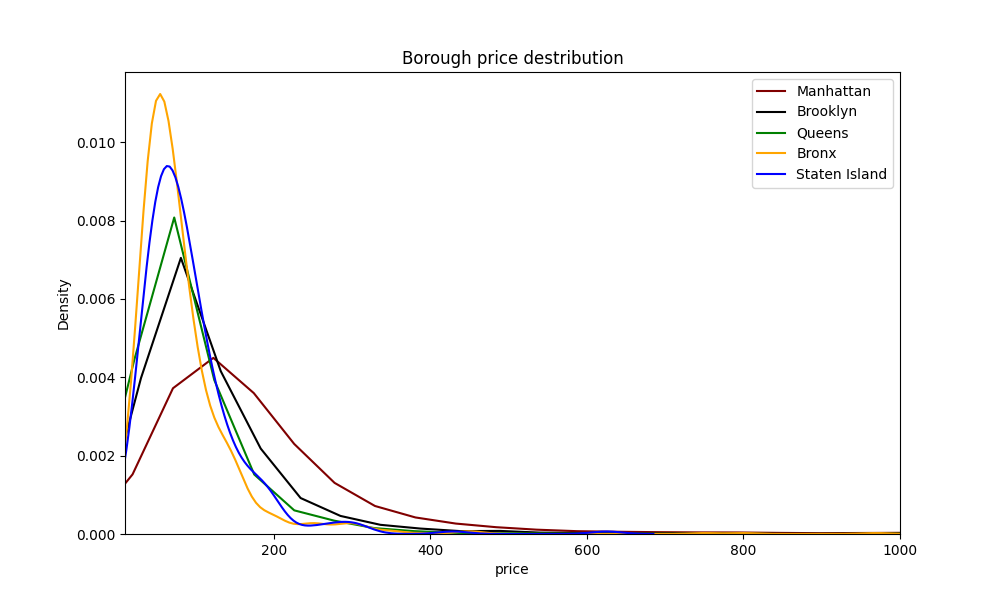
\includegraphics[width=\textwidth]{Figure_11_b.png}
    \caption{Borough Price Distribution}
    \label{fig:borough-price-distribution}
\end{figure}

\subsection{Property and room types}

As shown in Figure \ref{fig:property_type},
about 80\% properties are apartments. The remainder are houses or more uncommon
property types (e.g. 'bed and breakfast' or 'yurt').

\begin{figure}[H]
    \centering
    \begin{subfigure}[b]{0.48\textwidth}
        \centering
        \caption{Property Type Pie Chart}
        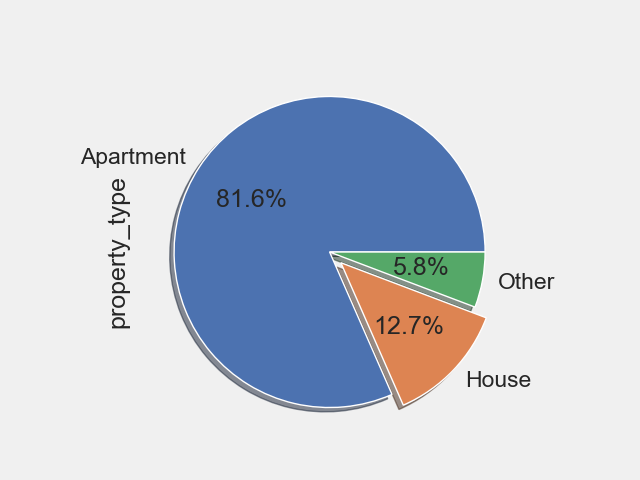
\includegraphics[width=\textwidth]{Figure_12_property_type_pie.png}
        \label{fig:property_type_pie}
    \end{subfigure}
    \begin{subfigure}[b]{0.48\textwidth}
        \centering
        \caption{Property Type Bar Chart}
        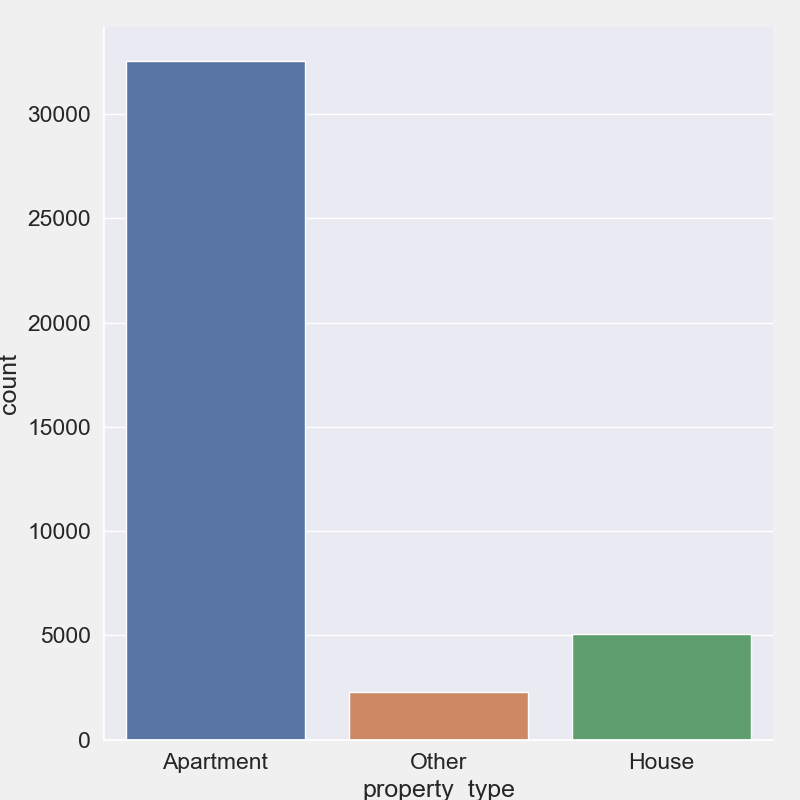
\includegraphics[width=\textwidth]{Figure_12_property_type.png}
        \label{fig:property_type_bar}
    \end{subfigure}

    \caption{Property Type}
    \label{fig:property_type}
\end{figure}


Lorem ipsum dolor sit amet, consetetur sadipscing elitr, sed diam nonumy eirmod
tempor invidunt ut labore et dolore magna aliquyam erat, sed diam voluptua. At
vero eos et accusam et justo duo dolores et ea rebum. Stet clita kasd gubergren,
no sea takimata sanctus est Lorem ipsum dolor sit amet.

\begin{figure}[H]
        \centering
        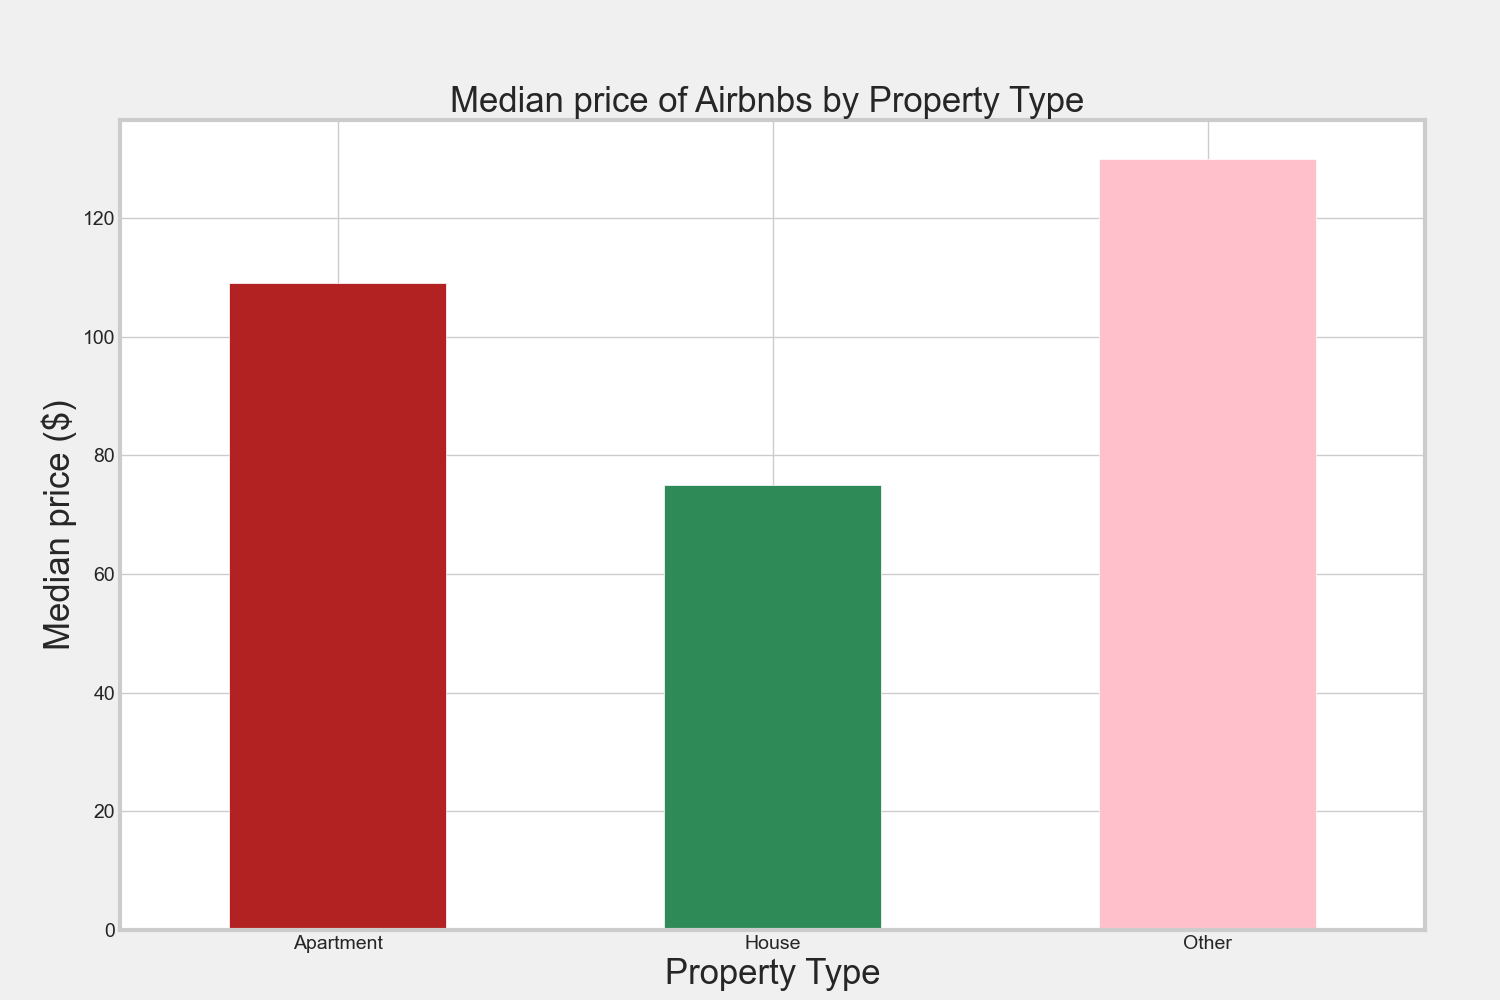
\includegraphics[width=0.75\textwidth]{Figure_12_property_type_price.png}
        \caption{Median Price By Property Type}
        \label{fig:property_type_price}
\end{figure}

Figure \ref{fig:room_type} shows that about 52\% of listings are entire homes
(i.e. you are renting the entire property on your own). Most of the remainder
are private rooms (i.e. you are renting a bedroom and possibly also a bathroom,
but there will be other people in the property). Fewer than 3\% are shared rooms
(i.e. you are sharing a room with either the property owner or other guests).

\begin{figure}[H]
    \centering
    \begin{subfigure}[b]{0.48\textwidth}
        \centering
        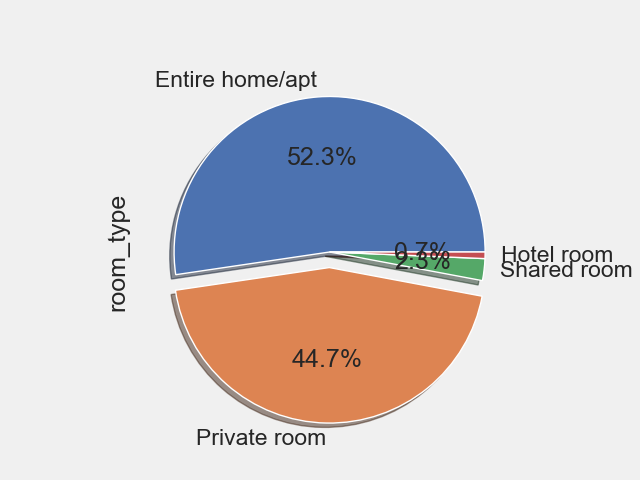
\includegraphics[width=\textwidth]{Figure_12_room_type_pie.png}
        \caption{Room Type Pie Chart}
        \label{fig:room_type_pie}
    \end{subfigure}
    \begin{subfigure}[b]{0.48\textwidth}
        \centering
        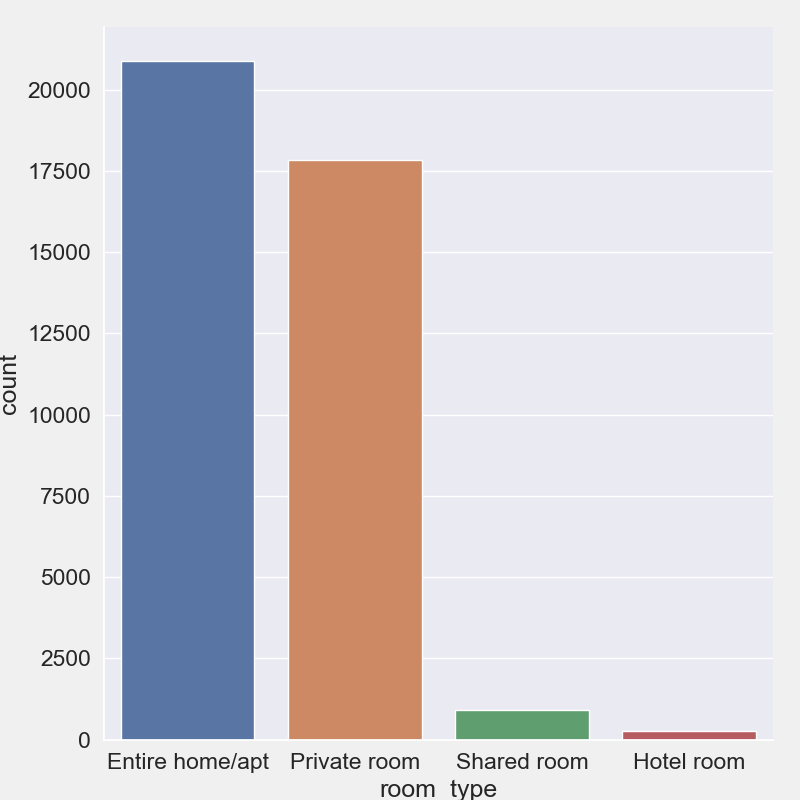
\includegraphics[width=\textwidth]{Figure_12_room_type.png}
        \caption{Room Type Bar Chart}
        \label{fig:room_type_bar}
    \end{subfigure}
    \caption{Room Type}
    \label{fig:room_type}
\end{figure}

On the question of whether there's a price difference between different types of
rooms, Figure \ref{fig:room_type_price} reveals that the rental price of the
entire home and a private room, and a hotel room is higher than the shared room.
This finding is consistent with many recent studies (\cite{cai2019price} ;
\cite{benitez2018flexible}; \cite{chen2017consumer}; \cite{gibbs2018use})

\begin{figure}[H]
        \centering
        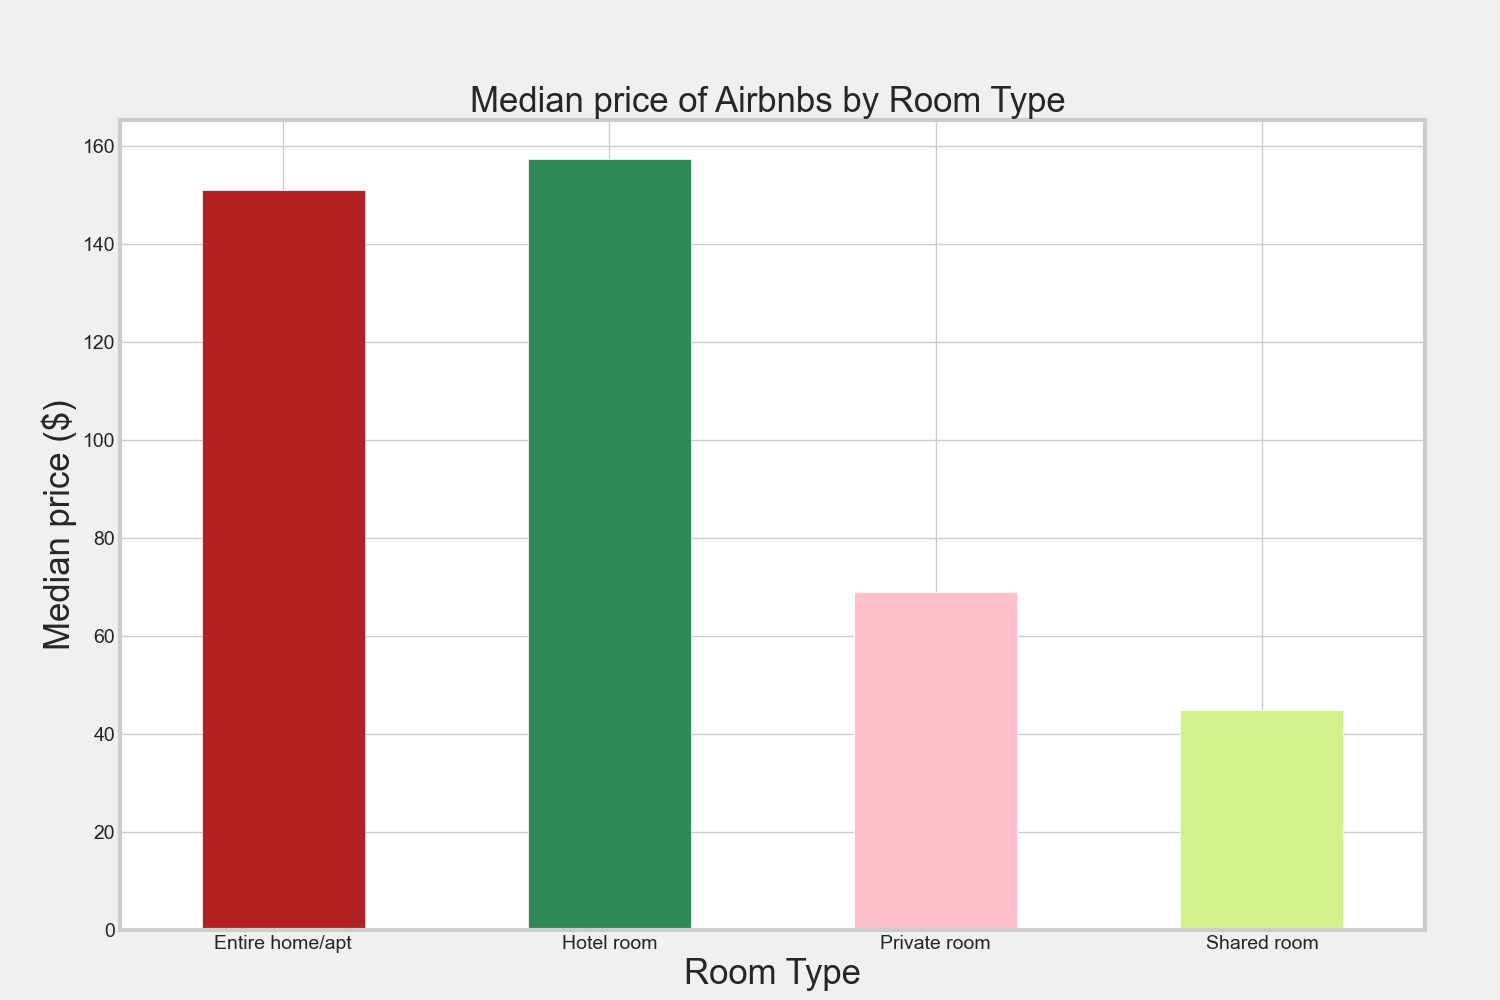
\includegraphics[width=0.75\textwidth]{Figure_12_room_type_price.png}
        \caption{Median Price By Room Type}
        \label{fig:room_type_price}
\end{figure}

\subsection{Reviews}

From Figure   \ref{fig:overall-listing}, we see that, while few listings receive
review ratings of 80 or below, most listings with a review have received a
95-100/100 overall,  indicating that the customers adore their Airbnbs.

\begin{figure}[H]\centering
    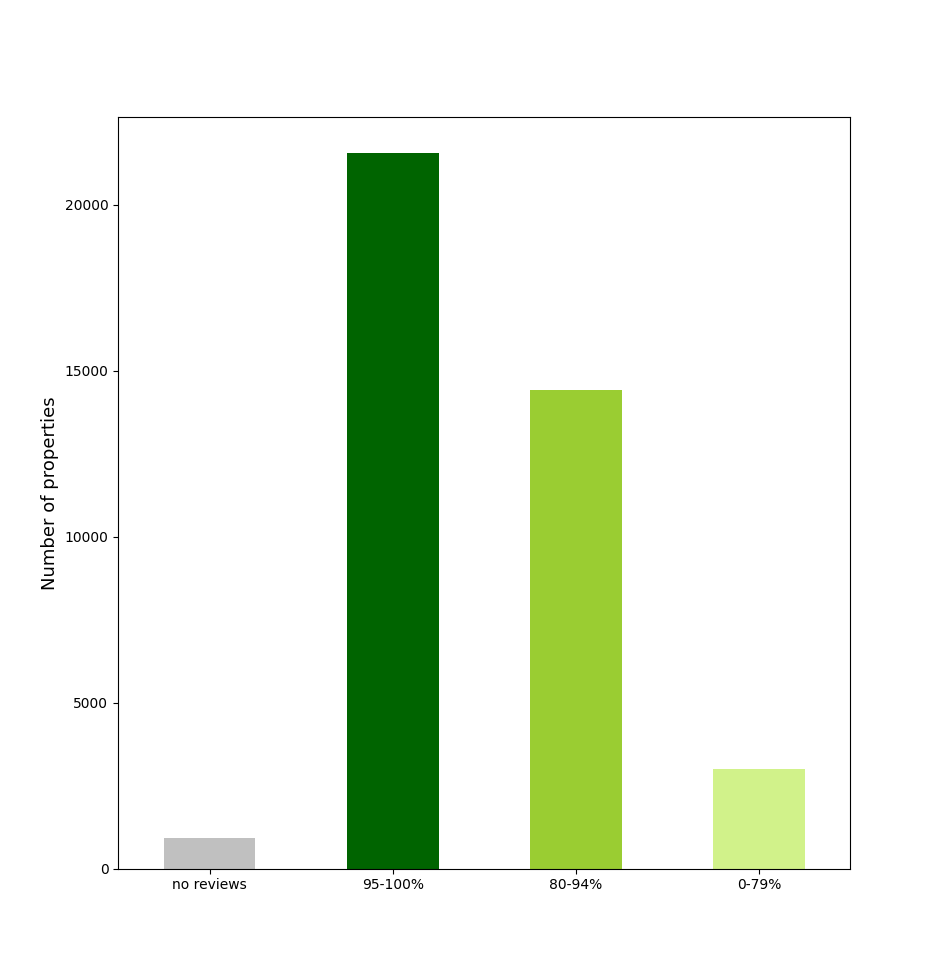
\includegraphics[width=0.60\textwidth]{Figure_13.png}
    \caption{Overall Listing Rating Distribution}
    \label{fig:overall-listing}
\end{figure}

As shown in Figure \ref{fig:price_by_review_score_rating}, the review score
rating has a positive effect on the median rental price. It all makes intuitive
sense customers are willing to pay a premium price for a listing with a good
reputation.  However, the evidence for the relationship between is inconclusive.
Many studies (\cite{chen2017consumer}; \cite{gibbs2018use};
\cite{wang2017price}) have shown that the overall rating score has a positive
impact on rental price, while others (\cite{li2016pros}; \cite{zhang2017key})
suggests the otherwise.

\begin{figure}[H]\centering
    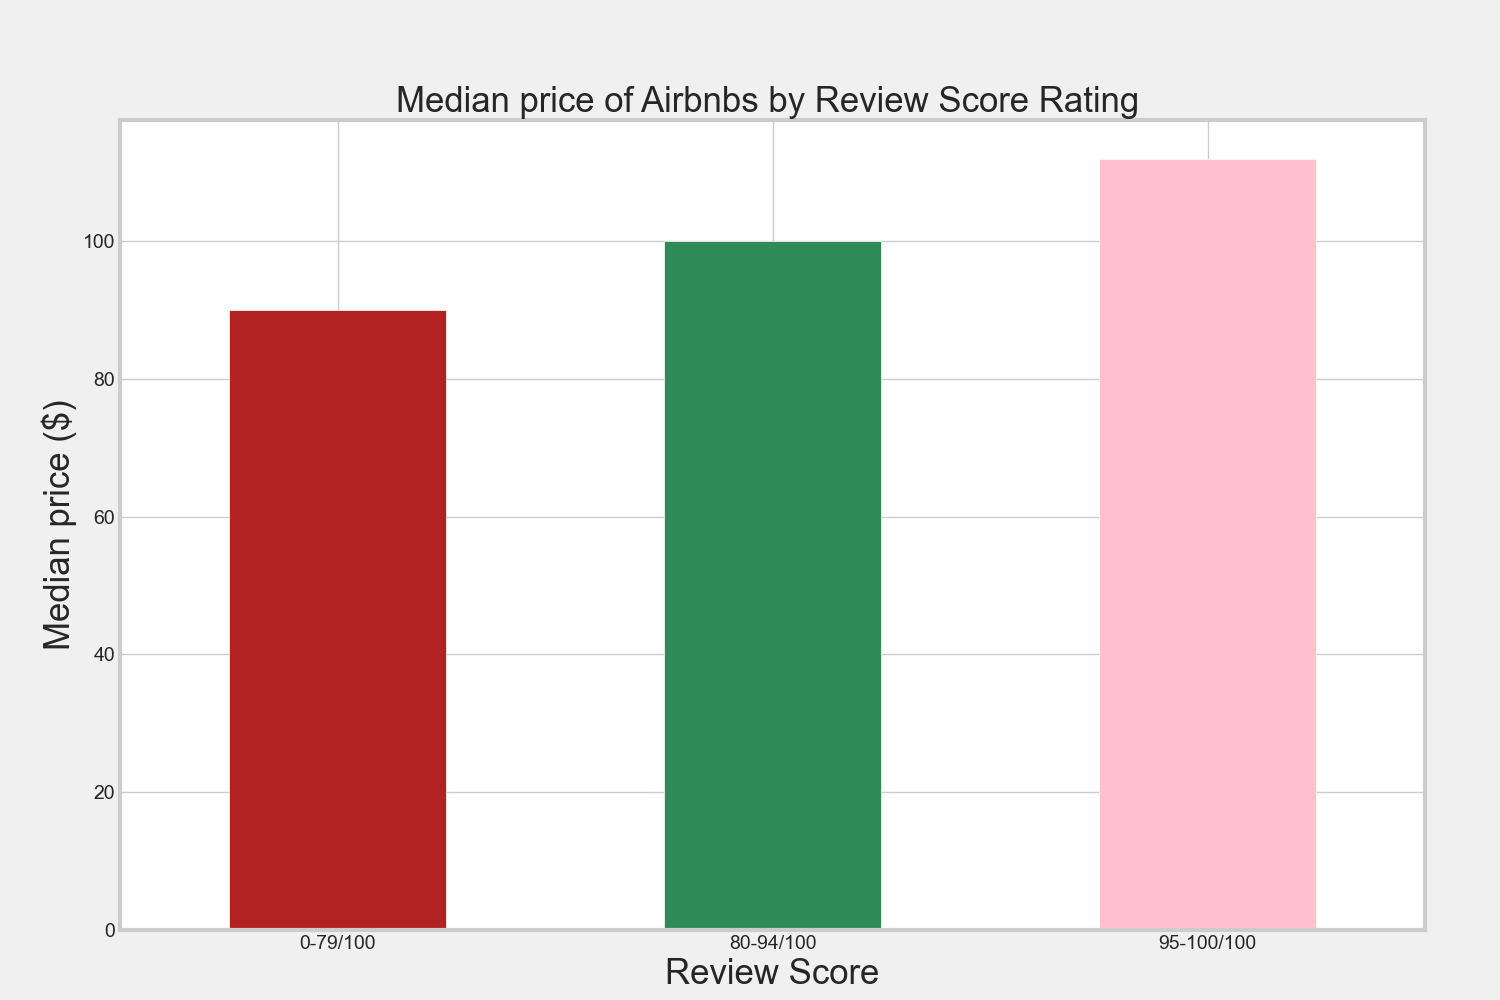
\includegraphics[width=0.60\textwidth]{Figure_13_review_score_price.png}
    \caption{Median Price By Review Score Rating}
    \label{fig:price_by_review_score_rating}
\end{figure}

\subsection{First and Last Review}

As can be seen from the Figure ~\ref{fig:time_since_first_review}, the most
common period in which  Airbnb listings had their first review is 2-3 years,
which means that many listings on the site have been active for at least a
couple of years. However,  fewer listings have been on Airbnb for more than four
years.

We expect that people would pay a higher price for listing lives in Airbnb for a
long time than listings with a recent history with Airbnb.
While the rental price is higher for listings had their reviews for four years
or more, there's no difference in median price for other categories
(\ref{fig:time_since_first_review_price})

\begin{figure}[H]
    \centering
    \begin{subfigure}[b]{0.48\textwidth}
        \centering
        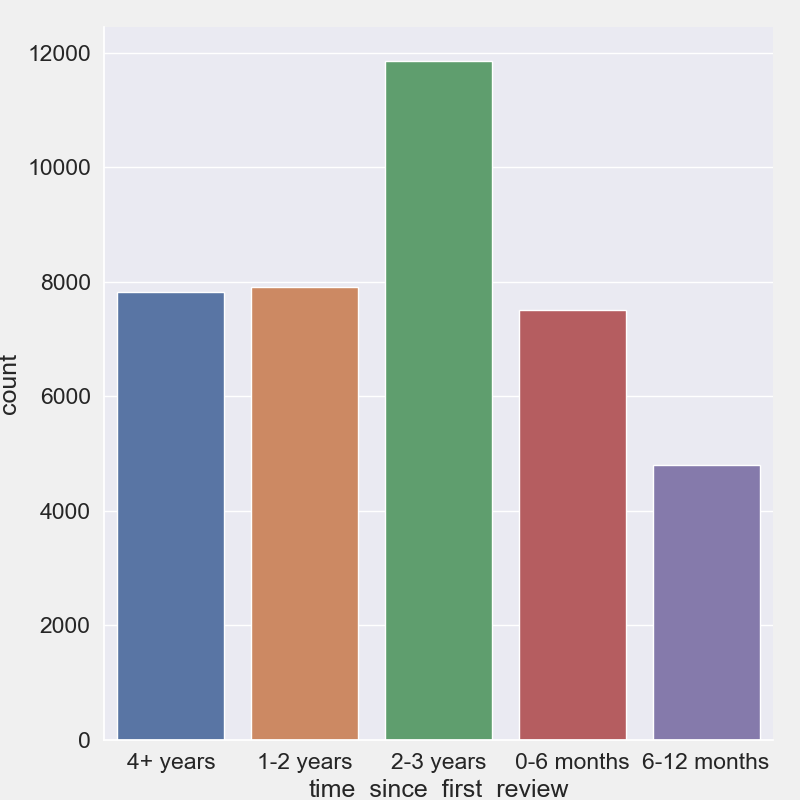
\includegraphics[width=\textwidth]{Figure_15_time_since_first_review.png}
        \caption{Time Since First Review}
        \label{fig:time_since_first_review}
    \end{subfigure}
    \begin{subfigure}[b]{0.48\textwidth}
        \centering
        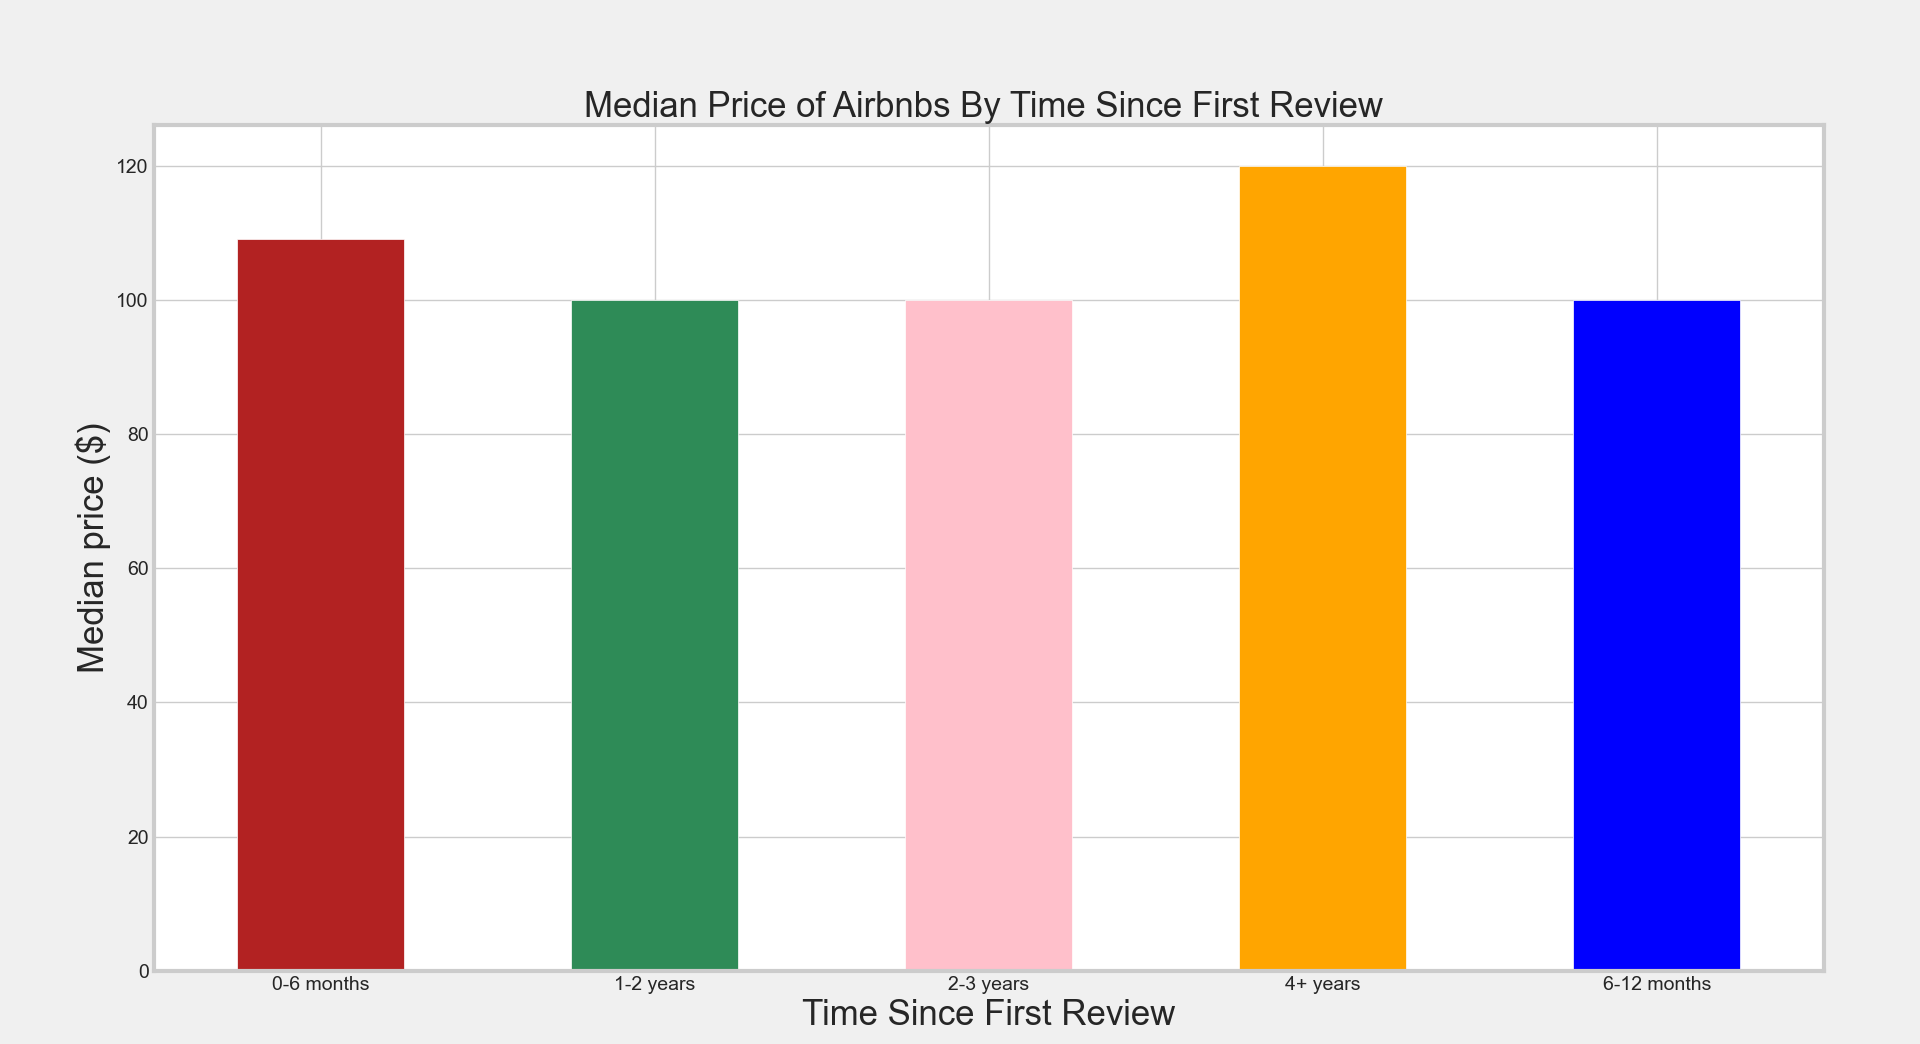
\includegraphics[width=\textwidth]{Figure_15_price_by_time_since_first_review.png}
        \caption{Median Price By Time Since First Review}
        \label{fig:time_since_first_review_price}
    \end{subfigure}
    \caption{Time Since First Review}
\end{figure}

The bar plot ~\ref{fig:time_since_last_review} reveals that the most
common period since a listing received its last review is 2-8 weeks, which means
that many listings have been reviewed relatively recently.  What stands out in
the figure is that over 10,000 listings have not had a review for more than a
year, which means they exist on the site, but they do not have their calendars
open and are not available to reserve.

Time since the last review may have been an essential factor in how people
decide to rent an Airbnb listing. People may avoid booking accommodation that
has not been reviewed for a long time. Therefore, we expect the time since the
last review has a negative effect on the rental price. Contrary to our
expectation, Figure \ref{fig:time_since_last_review_price} showed no significant
difference between different categories of the number of days since the last
review.

\begin{figure}[H]
    \centering
    \begin{subfigure}[b]{0.48\textwidth}
        \centering
        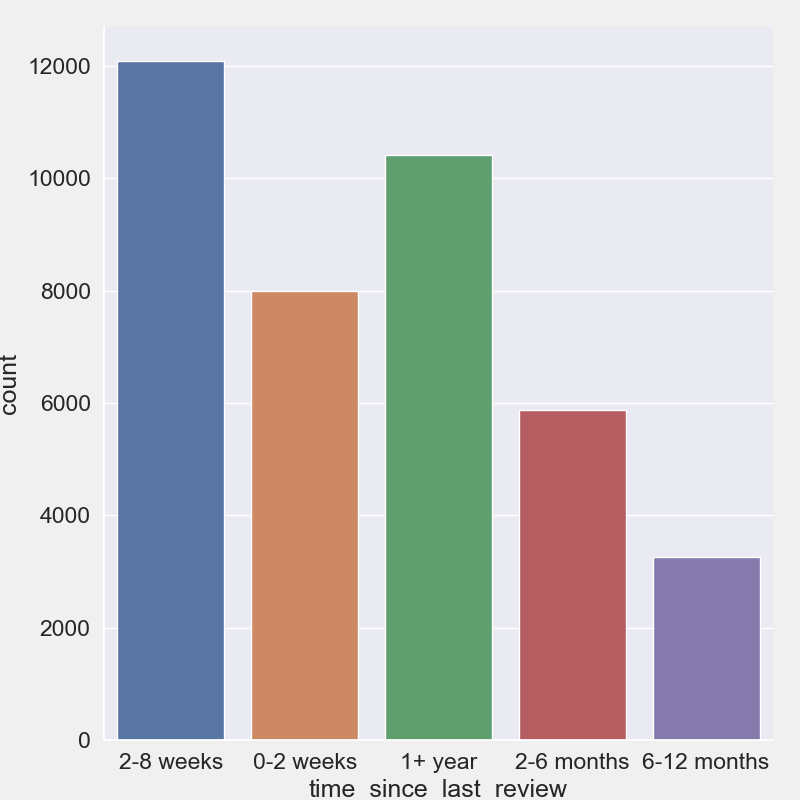
\includegraphics[width=\textwidth]{Figure_15_time_since_last_review.png}
        \caption{Time Since Last Review}
        \label{fig:time_since_last_review}
    \end{subfigure}
    \begin{subfigure}[b]{0.48\textwidth}
        \centering
        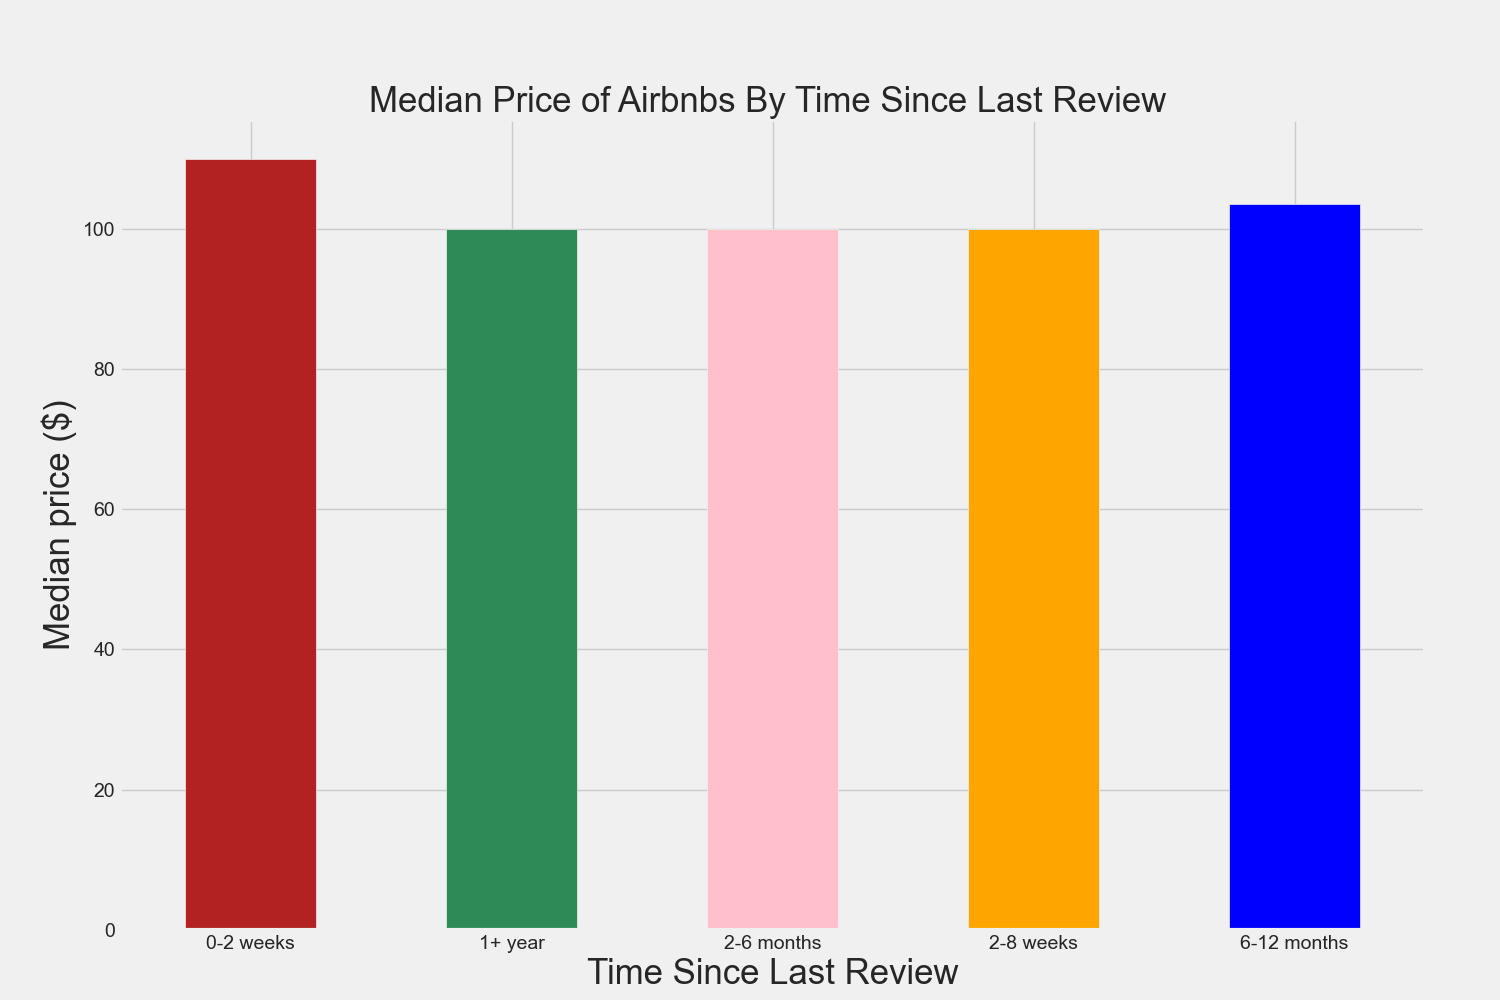
\includegraphics[width=\textwidth]{Figure_15_price_by_time_since_last_review.png}
        \caption{Median Price By Time Since Last Review}
        \label{fig:time_since_last_review_price}
    \end{subfigure}
    \caption{Time Since Last Review}
\end{figure}

\section{Boolean features}
\label{sec:boolean_features}

Many features (e.g. for amenities) can be true or false. This section compares
the proportions of these features that are true or false (to explore the data
and also to ascertain whether the feature is worth retaining), and the median
price of each category (to explore the relationship between the category and
price).

\subsection{Superhosts}

Figure ~\ref{fig:host_is_superhost} shows that about 23\% of hosts have a
superhost badge. Hosts with superhost status usually charge higher prices. A
possible explanation for this might be that people are willing to pay a premium
price because they consider superhost status a mark of quality.  This also
accords with earlier studies(\cite{gibbs2018use},
\cite{kakar2016effects};\cite{wang2017price},\cite{cai2019price}).

\begin{figure}[H]\centering
    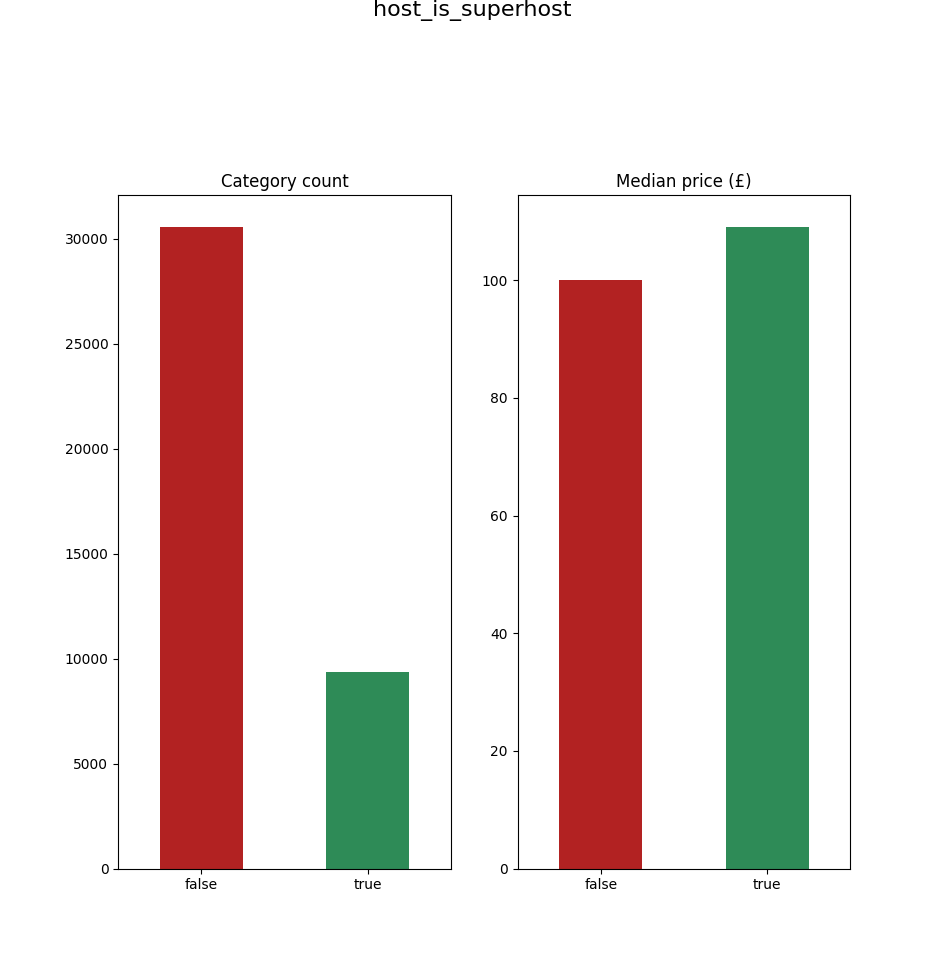
\includegraphics[width=0.45\textwidth]{Figure_16_host_is_superhost.png}
    \caption{host\_is\_superhost}
    \label{fig:host_is_superhost}
\end{figure}

\subsection{Host verification}
In Figure ~\ref{fig:host_identity_verified}, about 49\% of hosts are verified.
Consistent with the literature (\cite{chen2017consumer}; \cite{wang2017price}),
the figure showed that hosts with verified profiles gain a price premium. The
relationship may be explained by the fact that verified profiles (e.g., by
providing ID and verifying your phone number and email address)  can increase
their trustworthiness and, therefore, can charge a higher rental price.

\begin{figure}[H]
    \centering
    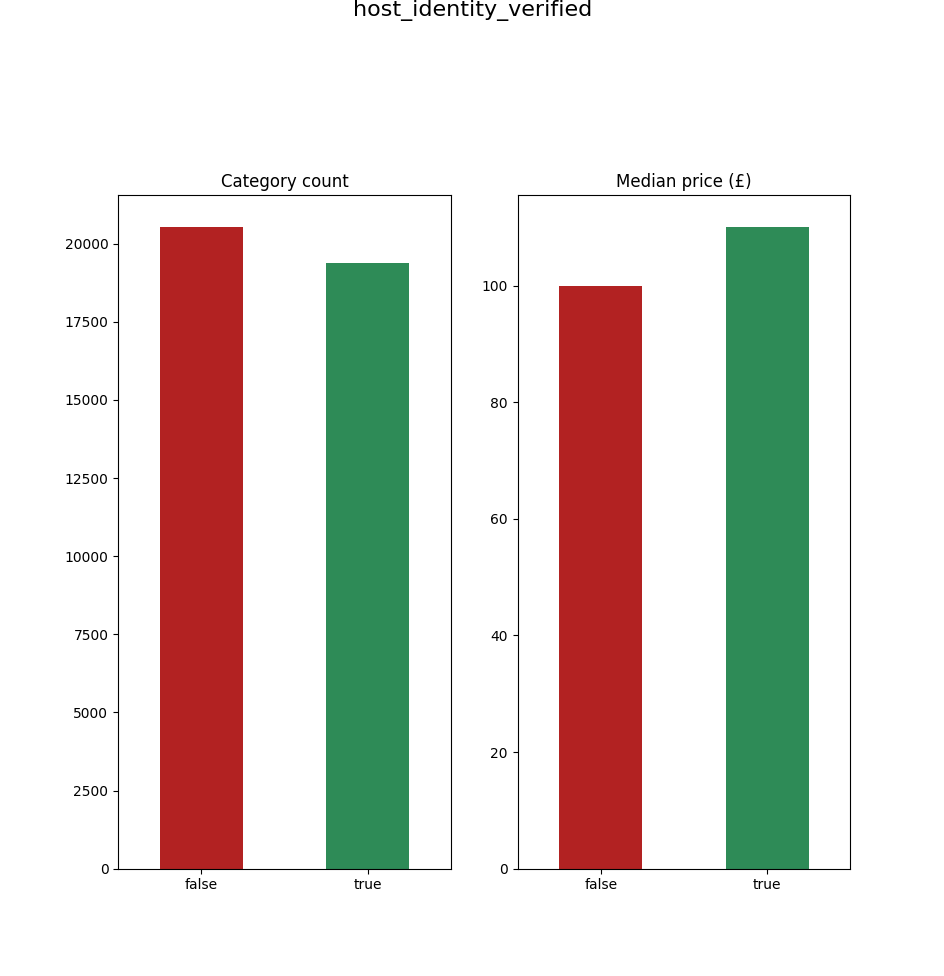
\includegraphics[width=0.45\textwidth]{Figure_16_host_identity_verified.png}
    \caption{host\_identity\_verified}
    \label{fig:host_identity_verified}
\end{figure}

\subsection{Instant booking}

As shown in figure below, about 40\% of properties are instant bookable and
hosts that allow for immediate booking without confirmation  have lower prices
than those who do not. This finding seems counterintuitive, as we would expect
higher willingness-to-pay from potential guests for the added convinience of
intant booking.  This negative link can be explained by both emotional
(\textcite{wang2017price}) and economic (\textcite{benitez2018flexible}).

\begin{figure}[H]
    \centering
    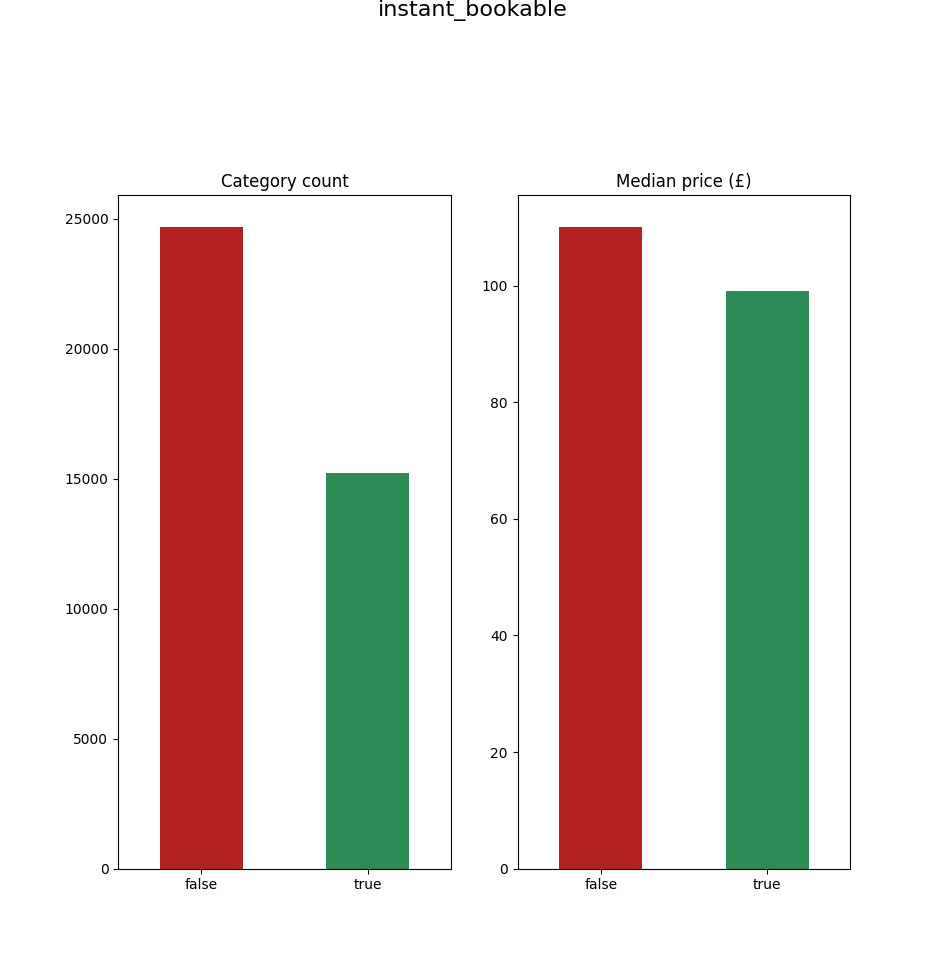
\includegraphics[width=0.45\textwidth]{Figure_16_instant_bookable.png}
    \caption{instant\_bookable}
    \label{fig:instant_bookable}
\end{figure}

\subsection{Amenities}

Our goal is to identify which amenities are common and which increase the price
of an Airbnb listing. We plot the count plot and each amenity's
median price to explore the relationship between the amenity and price.
Amenities then can be split into three groups:

\begin{enumerate}

  \item The first group contains uncommon amenity, but listings with it have a
    higher median price: Bed linen, Coffee machine, Basic cooking equipment,
    Elevator, Child friendly, Long term stays allowed, Private entrance, Self
    check-in, Pets allowed, Washer,dryer and/or dishwasher (white goods), Air
    conditioner.(See Figure ~\ref{fig:amenities-group1})

  \item The second group includes common amenities and listings with it have a
      higher median price: TV, Internet, Air conditioner (See Figure
      ~\ref{fig:amenities-group2}).

  \item The third group comprises uncommon amenities, and listings with it have
      a lower median price:  free car parking (presumably because these are less
      likely to be central properties), greeted by host. (See Figure
      ~\ref{fig:amenities-group3})

\end{enumerate}

It is somewhat surprising that free car parking does not have a significant
influence on the rental price. This may be because the more comfortable way and
quickest way to travel around New York City is by the subway, so people would
not consider car parking a critical factor when deciding to rent an Airbnb
listing. The reason why the host greeting does not associate with a higher price
is not apparent.

\section{Multivariate Exploration}
\label{sec:multivariate-exploration}

The goal of this section is to investigate the relationships between pairs of
our features. A primary concern when analyzing the relationship between various
variables is multicollinearity, a phenomenon in which two or more independent
variables substantially correlate(\textcite{cohen2013applied}).

While multicollinearity does not hurt the model's predictive
power(\textcite{kutner2005applied}), collinearity can pose problems in the
regression context. In particular,  it can be challenging to separate the
individual effects of collinear independent variables on the outcome variable.

A straightforward way to detect collinearity is to construct a correlation
matrix among predictors.  An element of this matrix that is large in absolute
value indicates a pair of highly correlated variables and are indicative of
collinearity issues.

\begin{figure}[H] \centering
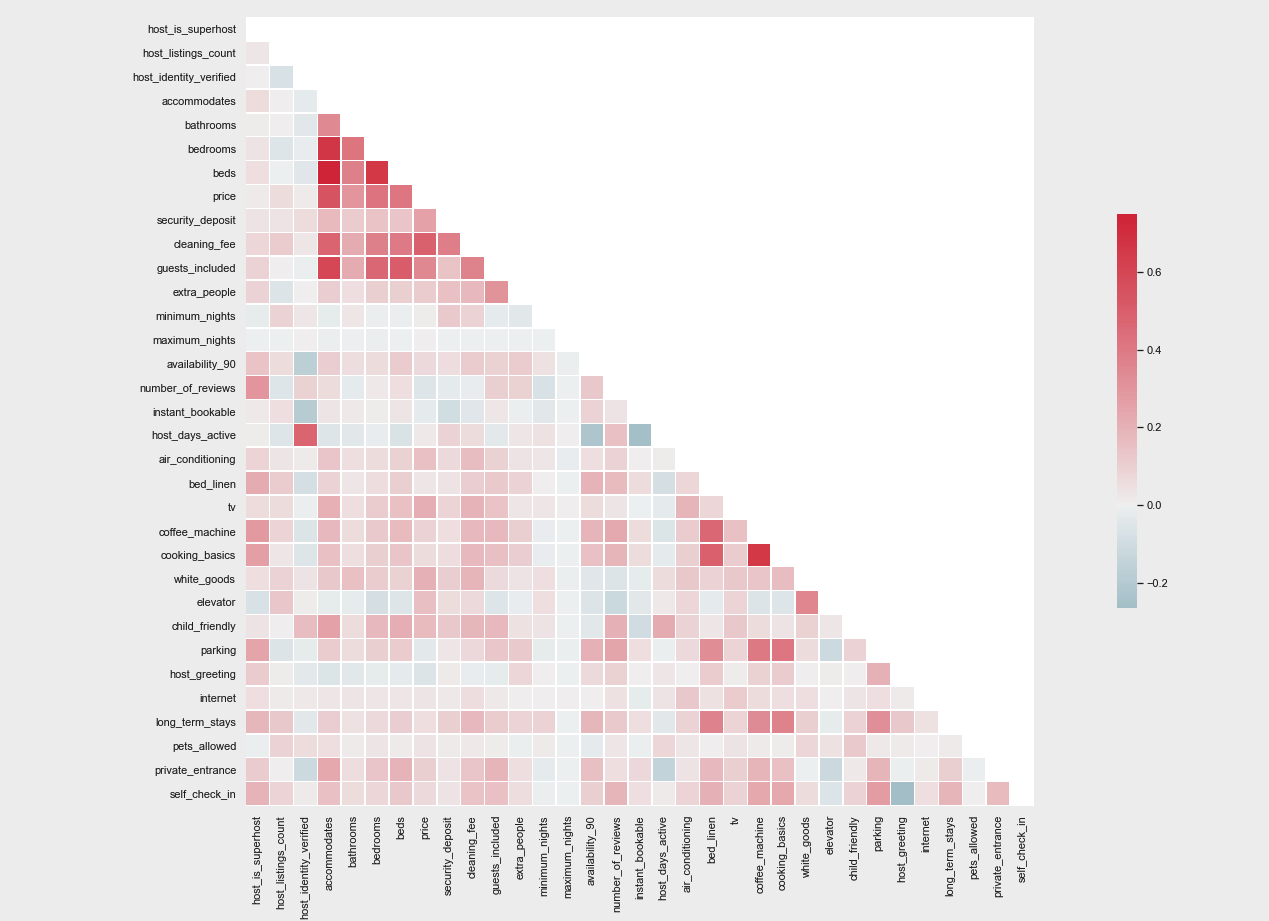
\includegraphics[width=\textwidth,keepaspectratio]{figures/correlation-matrix.png}
\caption{Correlation Matrix}
\label{fig:correlation-matrix}
\end{figure}

As shown in Figure ~\ref{fig:correlation-matrix} shows the correlation matrix,
areas of multicollinearity are:
\begin{itemize}
    \item As discussed in \ref{sec:numerical_features},
        Beds, bedrooms, guests included, and the number of people that property
        accommodates are highly correlated.
    \item There are strong negative correlations between houses and apartments
        and between private rooms and entire homes.
\end{itemize}

Providing a full remedy for the multicollinearity issue is beyond the scope of
this thesis. However, we employ two  simple approaches as followed:

\begin{enumerate}
    \item The first approach is to drop problematic variables from the regression.
    \item The second method is to employ regularization techniques, which combat
        collinearity by using biased models(\ref{sec:penalized_regression_models}),
        which reduce the error variance of estimators.
\end{enumerate}

\section{Time Series Analysis}
\label{sec:time_series}

We now also plotted time series charts to check for trends and seasonality.
First, we examine how long hosts have been listing properties on Airbnb in New
York.Of the Airbnb hosts that are active on the site, the first joined on 22
August 2008, and the most recent joined on 03 December 2019.
From 2011 onwards, the number of listings started growing considerably. However,
growth in the number of new hosts (of those currently listed on the site) has
decreased since mid-2014 (~\ref{fig:number_of_hosts_joining}).

Strong evidence of seasonality was found in Figure
~\ref{fig:number_of_hosts_joining}. The number of hosts joining Airbnb peaked in
the summer because people put properties online to utilize the increased number
of tourists in the summer holidays.


%\begin{figure}[H] \centering
%\caption{New York hosts joining Airbnb and listings getting their first review
%in each month}
    %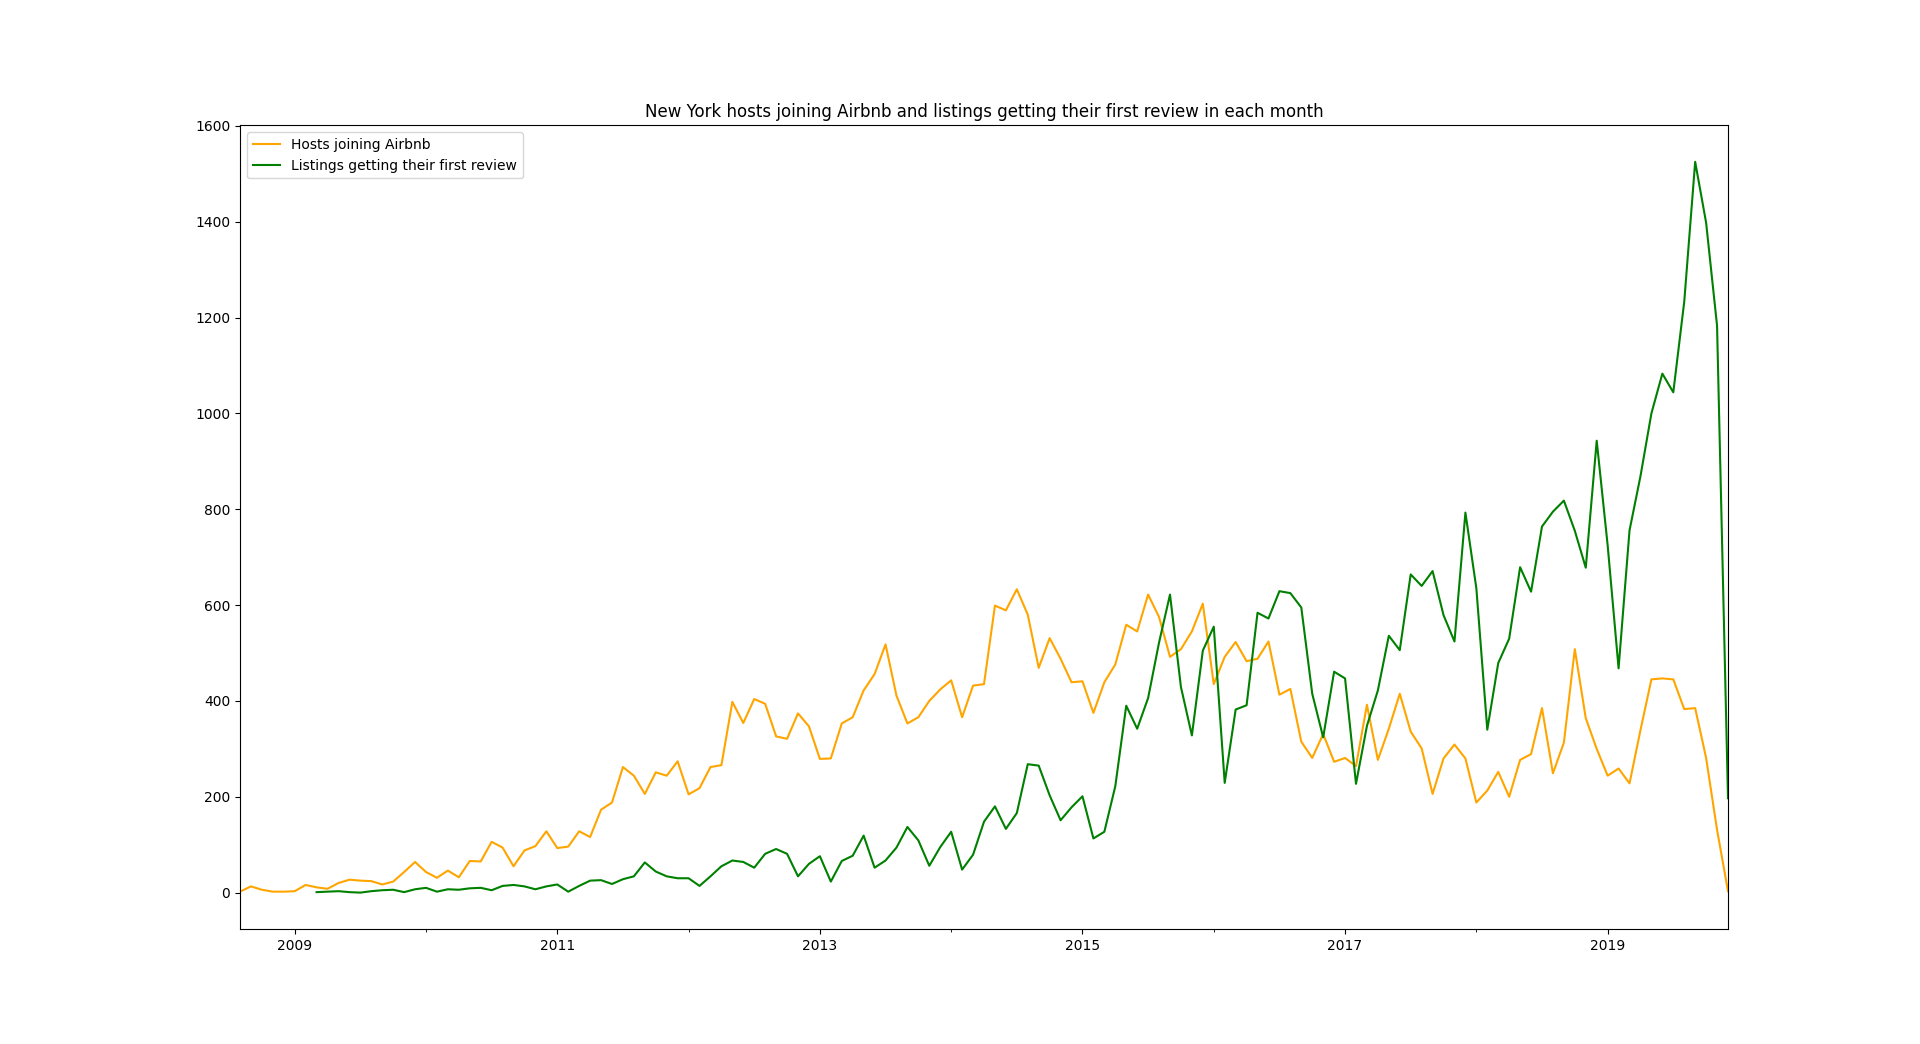
\includegraphics[width=\textwidth]{Figure_1.png}
    %\label{fig:number_of_airbnb_listing}
%\end{figure}


\begin{figure}[H] \centering
    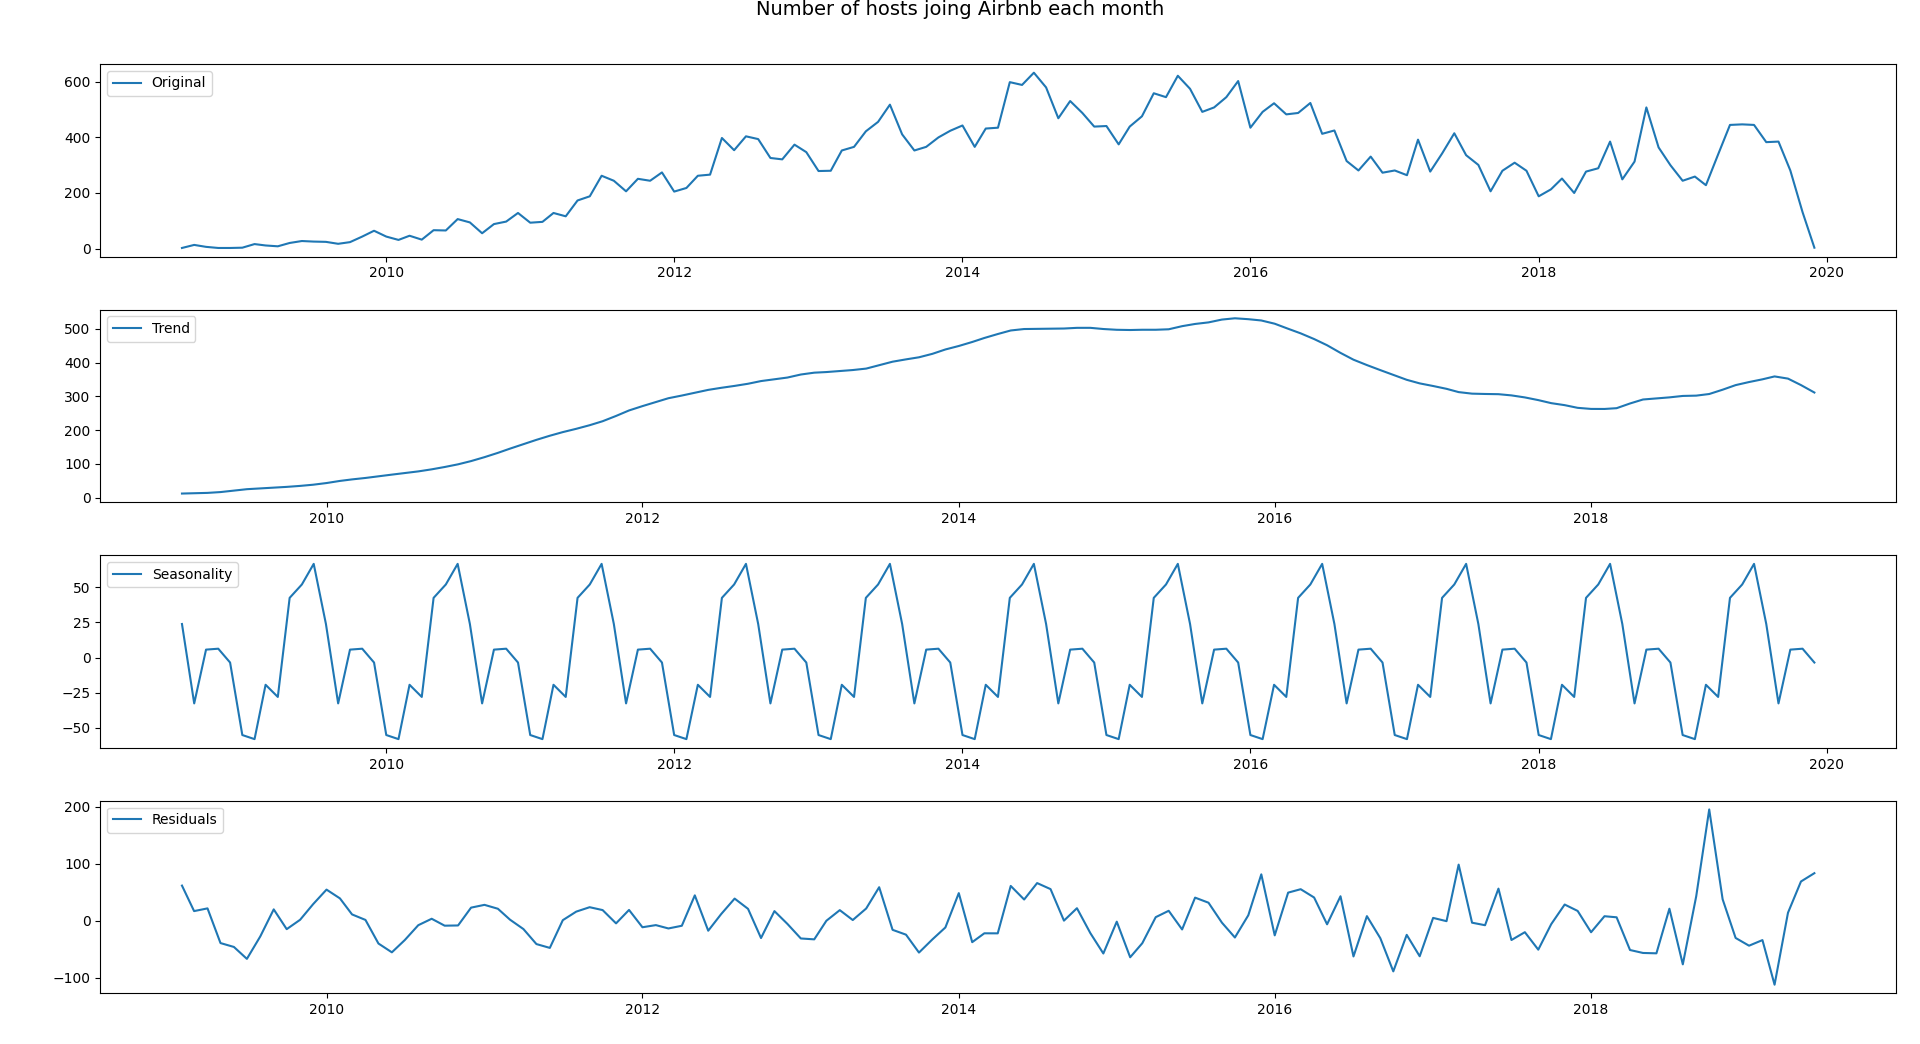
\includegraphics[width=\textwidth]{Figure_2.png}
    \caption{Number of hosts joining Airbnb each month}
    \label{fig:number_of_hosts_joining}
\end{figure}

%\begin{figure}[H] \centering
    %\caption{Number of Airbnb listings getting their first review each month}
    %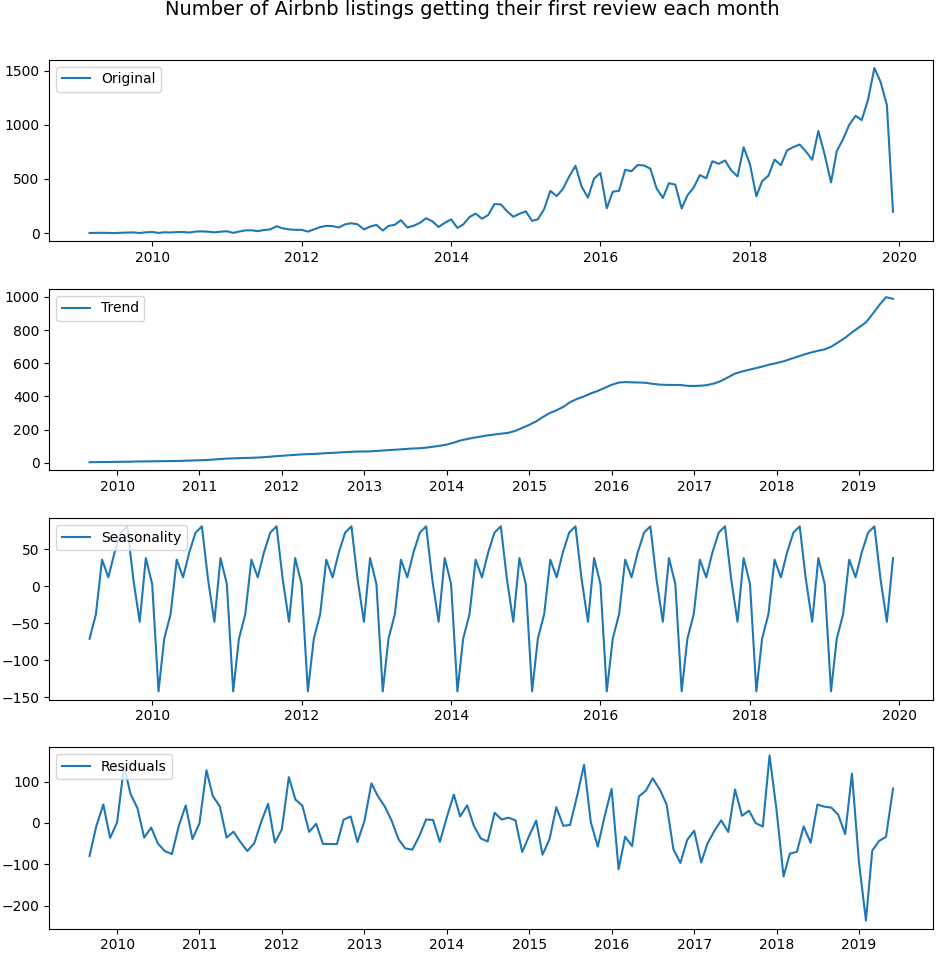
\includegraphics[width=\textwidth]{Figure_3.png}
    %\label{}
%\end{figure}

%\begin{figure}[H] \centering
%\caption{Change per year in the number of listings per host on Airbnb in New
%York}
    %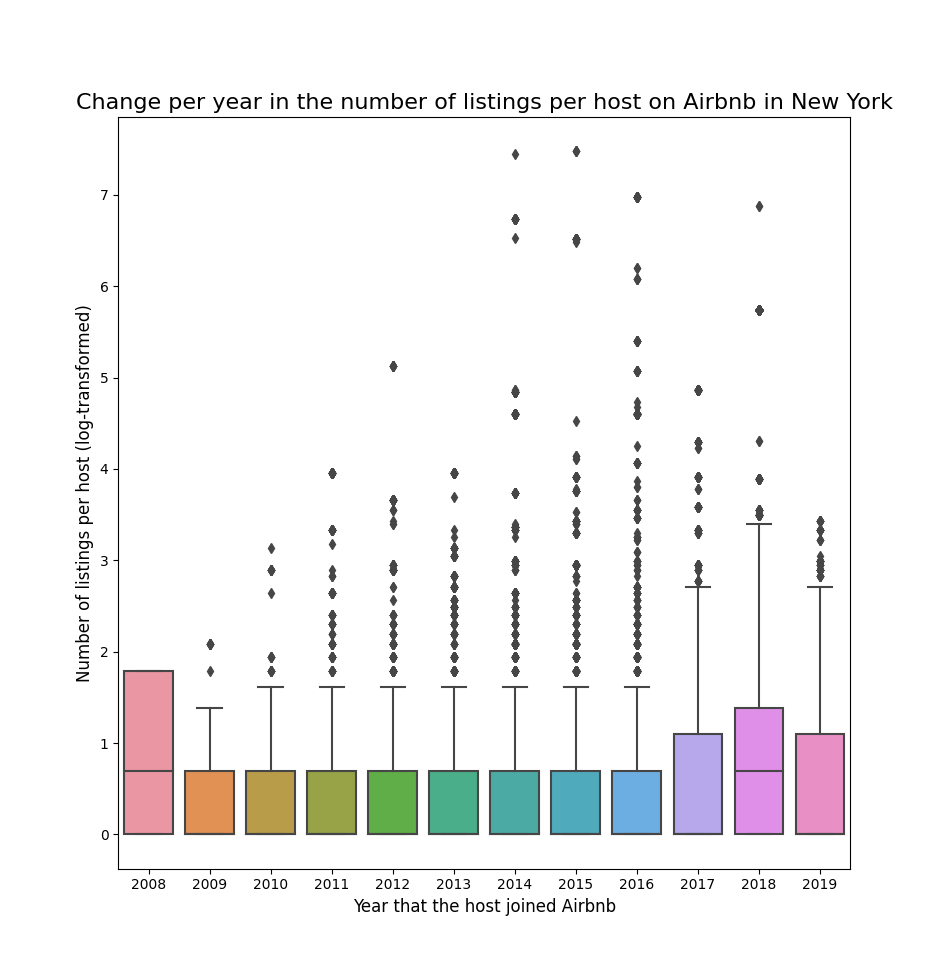
\includegraphics[width=\textwidth]{Figure_4.png}
%\end{figure}

In terms of how prices changed over time, Figure
~\ref{fig:prices-change-by-years} shows that the average price per night for
Airbnb listings in New York has increased slightly over the
last ten years. Particularly, the top-tier property prices have increased,
resulting in a more substantial increase in the mean price than the median.

\begin{figure}[H] \centering
    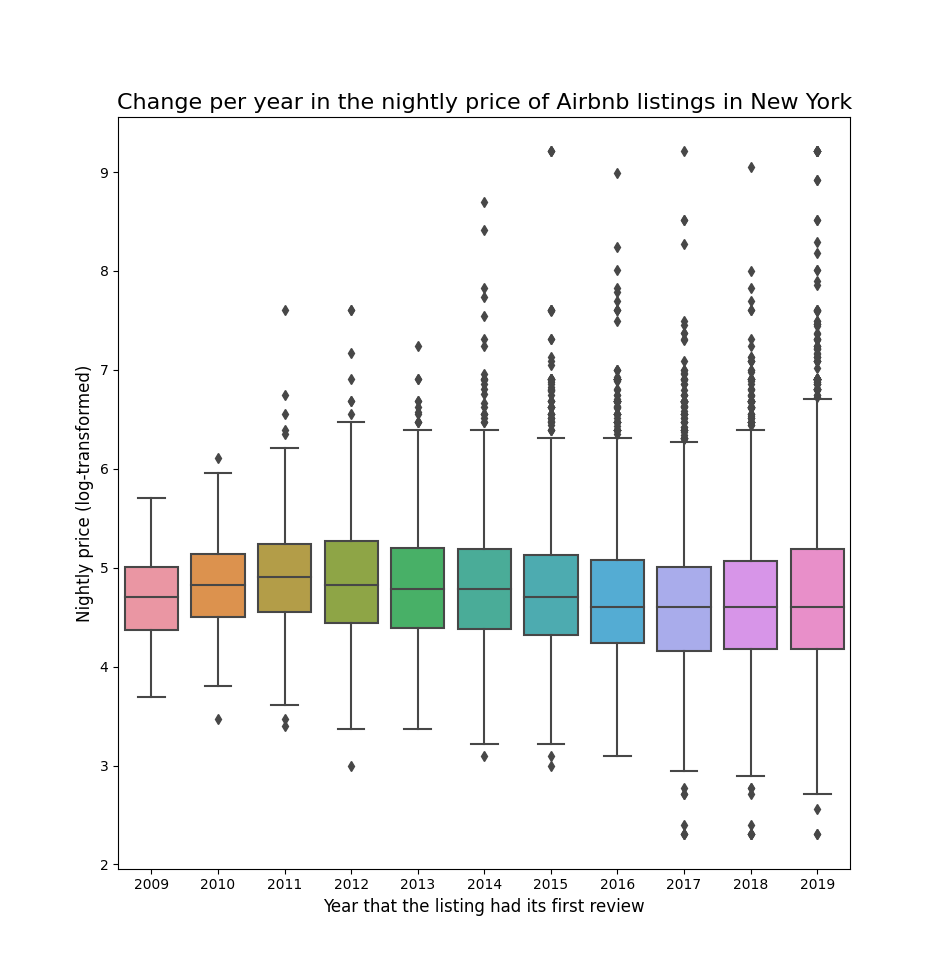
\includegraphics[width=0.75\textwidth]{Figure_5.png}
    \caption{Change per year in the nightly price of Airbnb listings in New York}
    \label{fig:prices-change-by-years}
\end{figure}

%Question: how long have hosts been listing properties on Airbnb in London?
